\documentclass[]{FZGdasa}
% {Klassen} entspr. *.cls Dateien:
% FZGdasa > arbeitet mit \chapter als höchste Ebene
%
% [Optionen]:
% entwurf      > Erstelldatum, Anmerkungen usw. sichtbar
% notoc        > kein Inhaltsverzeichnis
% nokeys       > keine labels anzeigen im entwurf-Modus
% notodolist   > keine Auflistung der mit \Note \sNote \Explain \Reminder \sReminder gekennzeichneten Stellen
% noxurl       > kein Zeilenumbruch in URL an alphanumerischen Zeichen, aber Skalierung des Zeichenabstands in URL in Literaturverzeichnis
% english

% Schlüsselwörter:
\Arbeit{Semesterarbeit}
\Nummer{16}
\ThemaDeutsch{Berechnung und experimentelle Untersuchung der Zahnfußspannung kurzfaserverstärkter Kunststoffzahnräder}
% \ThemaEnglisch{Titel in Englisch (entfällt bei Semesterarbeit)}
\ErlangungGrad{M.Sc.}
\AutorAnrede{Herr}
\Autorname{Tim Kuhn}
\AutorMatrNr{03738470}
\Betreuername{Liang Wang}
\Themenstellername[Prof. Dr.-Ing.]{Karsten Stahl}
\ThemenstellerZusatz{Lehrstuhl für Maschinenelemente}
\Beginn{27.04.2026}
\Ende{27.10.2026}
\Ort{Garching bei München}
\Aufgabepfad{aufgabenstellung.tex}

% Verfügbare Kommandos:
%\siehe[1]{s.~#1}
%{\chapref}[1]{\textbf{\chaptername~\ref{#1}}}
%{\schapref}[1]{\siehe{\chapref{#1}}}
%{\secref}[1]{\textbf{Abschnitt~\ref{#1}}}
%{\ssecref}[1]{\siehe{\secref{#1}}}
%{\eqref}[1]{\textbf{Formel~(\ref{#1})}}
%{\seqref}[1]{\siehe{\eqref{#1}}}
%{\figref}[1]{\textbf{\figurename~\ref{#1}}}
%{\sfigref}[1]{\siehe{\figref{#1}}}
%{\tabref}[1]{\textbf{\tablename~\ref{#1}}}
%{\stabref}[1]{\siehe{\tabref{#1}}}
%{\datref}[1]{\textbf{Dateifenster~\ref{#1}}}
%{\sdatref}[1]{\siehe{\datef{#1}}}

%\addbibresource{litbib.bib}

\begin{document}

%==== Kap1: ====
\chapter{Einleitung}
\label{sec:Einleitung}

Die vorliegende Untersuchung befasst sich mit der numerischen Simulation einer rechteckigen Scheibe, die durch eine zentrale elliptische Aussparung geschwächt wird. Die Geometrie ist durch eine horizontale Länge von ${l = 100\,\mathrm{mm}}$ und eine vertikale Höhe von ${h = 40\,\mathrm{mm}}$ charakterisiert, wobei die zentrale Ellipse Halbachsen von ${a = 6\,\mathrm{mm}}$ und ${b = 3\,\mathrm{mm}}$ aufweist. Um die mechanische Antwort unter einachsiger Belastung zu analysieren, wird das Modell an der linken Stirnfläche in ${x}$-Richtung eingespannt und an der gegenüberliegenden Seite mit einer Zugspannung von ${\sigma_0 = 100\,\mathrm{MPa}}$ beaufschlagt. Weiter wird der Freiheitsgrad in ${y}$-Richtung dir Lochscheibe an der Unterseite eingeschränkt.

Methodisch liegt der Fokus der Problemlösung auf einer Diskretisierungsstrategie, um trotz einer vorgegebenen Knotenobergrenze eine hinreichende Ergebnisgüte zu erzielen. Hierzu wird die Geometrie nach initialer Analyse mit einem unsortierten Netz zunächst gezielt in vier Quadranten partitioniert, um die Anwendung eines strukturierten Netzes zu ermöglichen. Das Vorgehen bei der Netzgenerierung konzentriert sich primär auf die lokale Verfeinerung am Ort der erwarteten Spannungskonzentration. Durch den Einsatz eines einseitigen Gradienten \texttt{Single Bias} wird die Knotendichte am Lochrand signifikant erhöht, während das Netz zu den Außenrändern hin sukzessive vergröbert wird. Ein wesentlicher Teil der Untersuchung widmet sich dabei der gezielten Auswahl der Elementformulierung. Hierbei wird insbesondere analysiert, inwieweit voll integrierte quadratische Elemente \texttt{CPS8} im Vergleich zu linearen Ansätzen geeignet sind, die komplexen Spannungsgradienten an der Kerbe präzise abzubilden und so eine Annäherung an die theoretischen Referenzwerte zu gewährleisten.

%==== Kap2: ====
\chapter{Theorie}
\label{sec:Theorie}

Die mathematische Beschreibung von Spannungsfeldern in der Umgebung geometrischer Diskontinuitäten ist eine fundamentale Fragestellung der Elastostatik. Jede Störung des Kraftflusses, wie sie durch Bohrungen oder Aussparungen hervorgerufen wird, führt lokal zu einer signifikanten Überhöhung der Nennspannung, die als Spannungskonzentration bezeichnet wird. Der Theorieteil wurde unter Zuhilfenahme folgender Literatur ausgearbeitet: \cite{Niemann19} \cite{Sedlacek09} \cite{roesler12}.


\section{Analytische Lösung nach Inglis}
\label{sec:Analytische Lösung nach Inglis}

Für die Untersuchung einer unendlich ausgedehnten, linear-elastischen Scheibe mit einem elliptischen Loch unter einachsiger Zugbelastung stellt die Lösung nach Inglis die theoretische Referenz dar. Die maximale Normalspannung ${\sigma_{xx}^{\mathrm{P}}}$ tritt dabei stets an den Scheitelpunkten der Hauptachse auf, die senkrecht zur Lastrichtung orientiert ist. Diese berechnet sich in Abhängigkeit der Halbachsen ${a}$ (vertikal) und ${b}$ (horizontal) nach der Beziehung:

\begin{equation}
    \sigma_{xx}^{\mathrm{P}} = \sigma_{0} \cdot \left( 1 + \frac{2a}{b} \right).
    \label{eq:Inglis Lösung}
\end{equation}

Hierbei definiert der Term ${\alpha_{\mathrm{k}} = \left( 1 + \frac{2a}{b} \right)}$ die theoretische Formzahl (Spannungskonzentrationsfaktor).

\section{Einfluss der Geometrie und Grenzfälle}
\label{sec:Einfluss der Geometrie und Grenzfälle}

Die analytische Gleichung verdeutlicht, dass die Spannungsüberhöhung maßgeblich vom Achsenverhältnis der Ellipse bestimmt wird. Hierbei lassen sich zwei physikalisch relevante Grenzfälle ableiten:

\begin{itemize}
    \item Kreisförmiges Loch: Für den Fall ${a = b}$ reduziert sich die Formzahl auf den konstanten Wert ${\alpha_{\mathrm{k}} = 3}$, was der klassischen Lösung nach Kirsch entspricht.
    \item Rissartiger Defekt: Nähert sich die horizontale Halbachse dem Wert ${b \rightarrow 0}$, strebt die theoretische Spannungsspitze gegen Unendlich (${\sigma_{xx}^{\mathrm{P}} \rightarrow \infty}$), was die Grundlage der Bruchmechanik hinsichtlich der Singularität an Risspitzen bildet.
\end{itemize}

Es ist anzumerken, dass die analytische Lösung die Annahme einer unendlich ausgedehnten Scheibe trifft. In der numerischen Simulation der vorliegenden endlichen Scheibengeometrie (${\text{Breite } l = 100\,\mathrm{mm}}$) können daher geringfügige Abweichungen auftreten, da die Interaktion zwischen dem lokalen Spannungsfeld der Kerbe und den äußeren Berandungen physikalisch berücksichtigt wird.

%==== Kap3: ====
\chapter{Lösungsansatz}
\label{sec:Lösungsansatz}

Die numerische Umsetzung erfolgt in Abaqus/CAE (Standard/Static) und orientiert sich an einem modularen Aufbau (s. \secref{sec:Abaqus .cae-file}), um die Reproduzierbarkeit der Simulation zu gewährleisten. Alle Eingaben wurden unter Berücksichtigung der Einheiten $\mathrm{mm,\ N,\ t,\ s,\ MPa}$ vorgenommen, um die Konsistenz mit den analytischen Berechnungen sicherzustellen. Eingebundene Visualisierungen und in TUM-Moodle eingereichte Ausgaben aus Abaqus sind entsprechend einheitenlos.

Die numerische Untersuchung wird in mehrere Phasen unterteilt, um den Einfluss der Diskretisierungsstrategie und der Elementformulierung auf die Ergebnisgenauigkeit systematisch zu erfassen.

\section{Basismodellierung und initiale Diskretisierung (Teilaufgabe \text{a)})}
\label{sec:Basismodellierung und initiale Diskretisierung}

In der ersten Phase wird die Grundgeometrie der Lochscheibe ohne spezifische Netzoptimierungen abgebildet. Für die Vernetzung wird ein globaler Instanz-Seed von ${2.5}$ gewählt. (\sfigref{fig:lin-unseeded_mesh}) Als Elementtyp kommen lineare Standard-Elemente ohne reduzierte Integration \texttt{CPS4} zum Einsatz. Dieser Ansatz dient als Referenz \texttt{Kuhn\_A2-2\_lin-unseeded.odb}, um die prozentuale Abweichung der Diskretisierung vom analytischen Idealwert zu quantifizieren.

\section{Iterative Netzoptimierung und Sensitivitätsanalyse (Teilaufgabe \text{b)})}
\label{sec:Iterative Netzoptimierung und Sensitivitätsanalyse}

Der Schwerpunkt der Untersuchung liegt auf der schrittweisen Verfeinerung des Modells unter Berücksichtigung einer lizenzbedingten Knotenobergrenze von ${1000}$ nodes. Dieser Prozess wird in drei wesentlichen Veränderungen durchgeführt:
\begin{itemize}
    \item \texttt{Kuhn\_A2-2\_lin-seeded.odb}: Zur Verbesserung der lokalen Auflösung wird ein spezifisches Seeding ohne Bias am Lochrand appliziert. Mittels strukturierter Netzsteuerungen (\texttt{Quad-Structured}) wird eine erste lokale Konzentration der Elemente im Kerbbereich erzielt, während die Elementformulierung zunächst linear beibehalten wird. (\sfigref{fig:lin-seeded_mesh})
    \item \texttt{Kuhn\_A2-2\_quad-seeded\_V1.odb}: In dieser Iteration erfolgt der Wechsel auf quadratische, voll integrierte Elemente \texttt{CPS8}. Da dieser Elementtyp eine höhere Anzahl an Integrationspunkten und Knoten pro Element aufweist, wird die globale Elementanzahl im Vergleich zum linearen Modell reduziert, um die Knotenobergrenze einzuhalten. Um dennoch eine hohe Genauigkeit zu erzielen, wird die Scheibe in Quadranten partitioniert. Dies ermöglicht ein \texttt{Single-Bias Seeding} am Lochrand, welches die Knoten gezielt entlang der erwarteten Spannungsgradienten konzentriert. (\sfigref{fig:quad-seeded_V1_mesh})
    \item \texttt{Kuhn\_A2-2\_quad-seeded\_V2.odb}: Zur Untersuchung der numerischen Stabilität wird eine Sensitivitätsanalyse der Steuerungsparameter durchgeführt. Hierbei wird das Verhältnis zwischen kleinster und größter Elementdistanz (Bias-Ratio) an den radialen Partitionierungen der Quadranten sowie der Außenkanten eingestellt, um die Grenzen der Konvergenz und den Einfluss der Elementverzerrung auf die Spannungsspitzen zu evaluieren. (\sfigref{fig:quad-seeded_V2_mesh})
\end{itemize}

\begin{figure}[htbp]
    \centering

    \begin{subfigure}{0.48\textwidth}
        \centering
        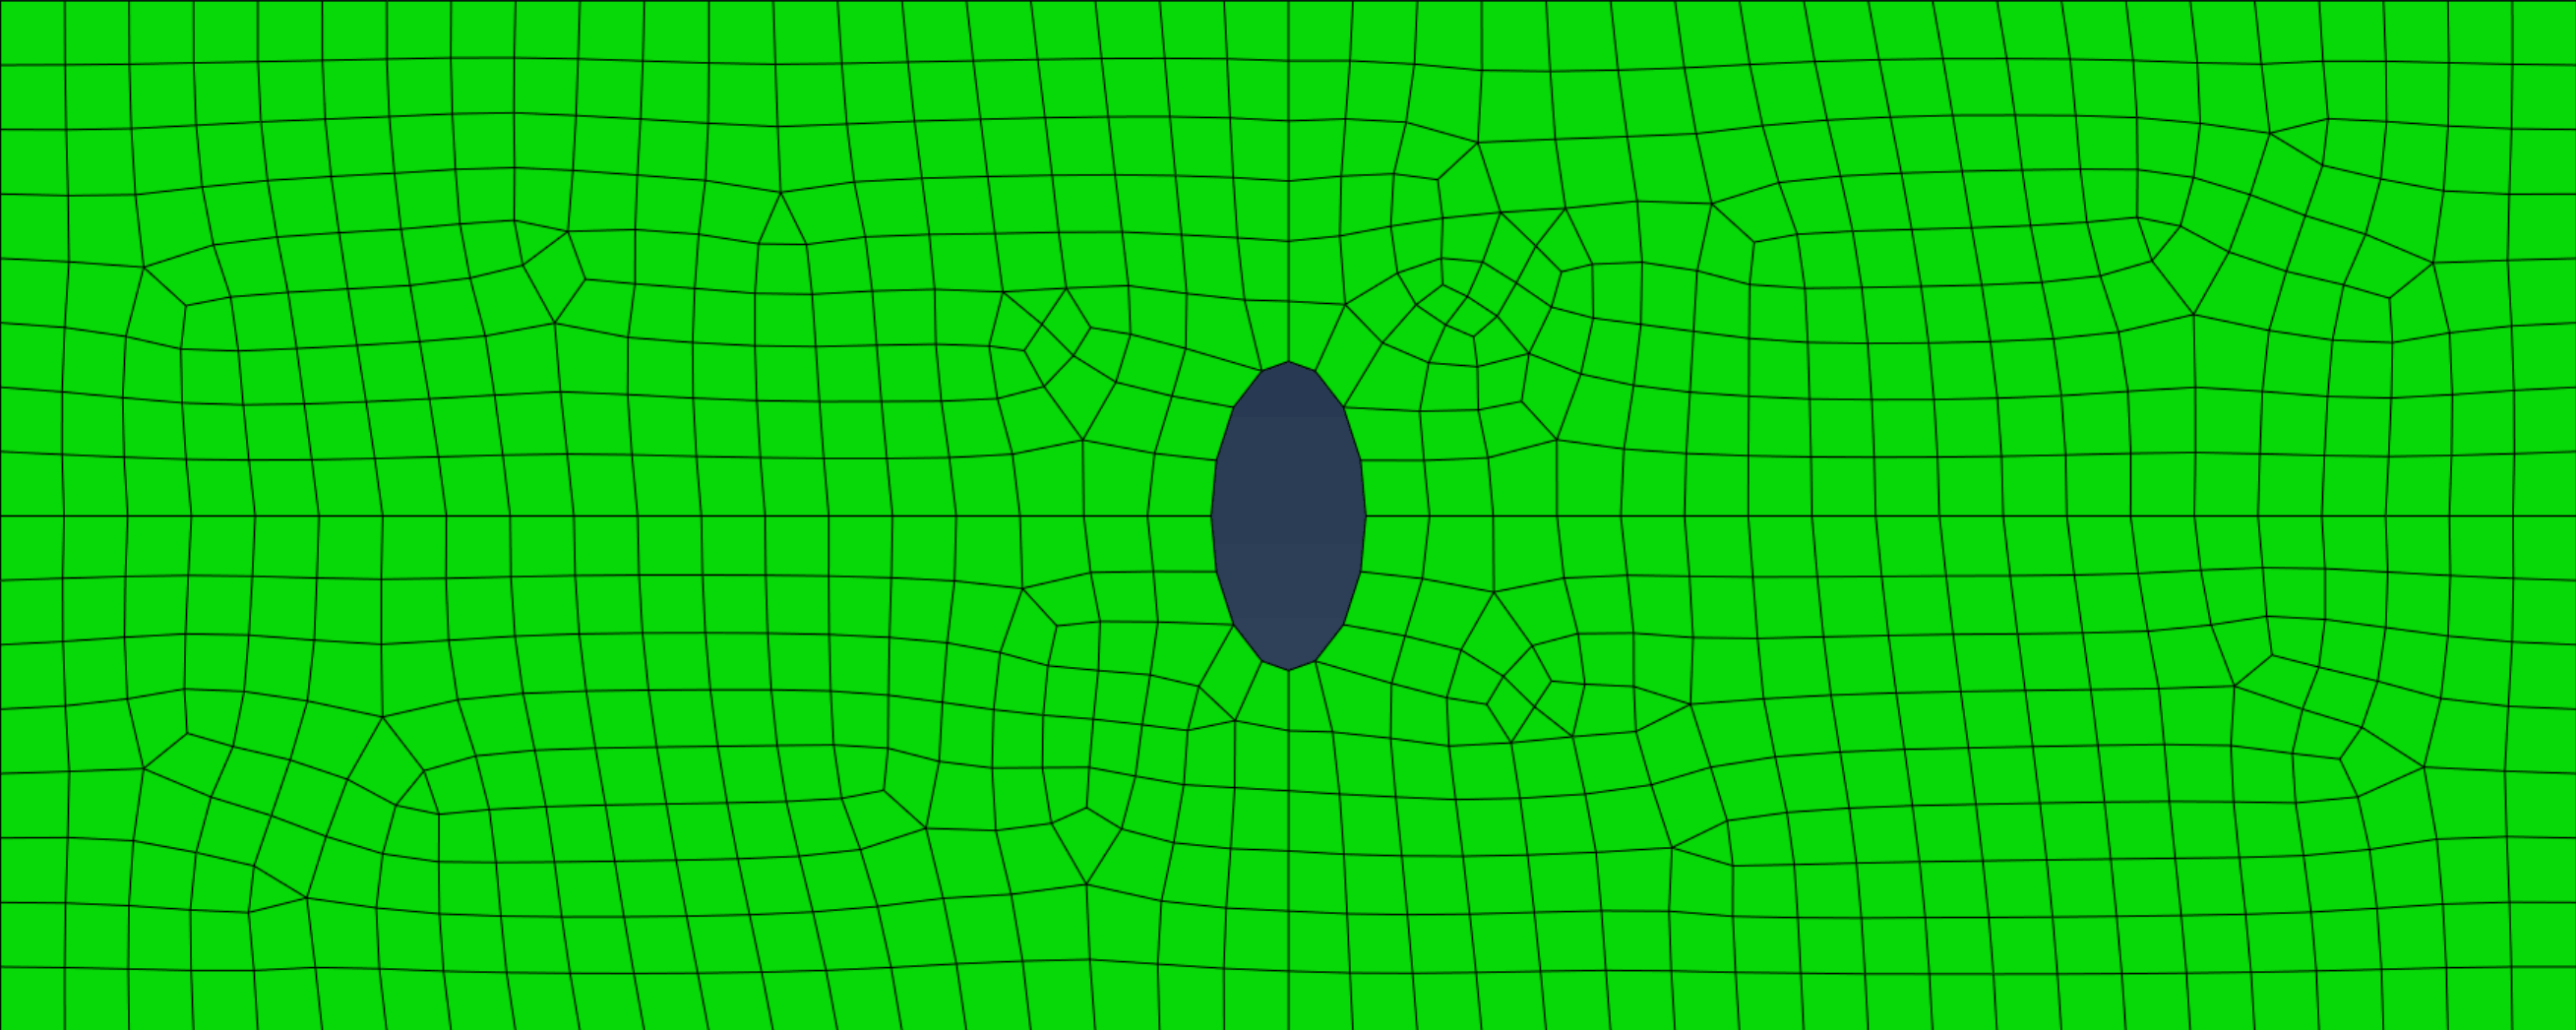
\includegraphics[width=\textwidth]{_ltx/Kuhn_A2-2_lin-unseeded_mesh.png} % Datei für unseeded mesh
        \caption{Mesh der Scheibe mit linearen Elementen und ungesteuertem Seeding}
        \label{fig:lin-unseeded_mesh}
    \end{subfigure}
    \hfill % Schiebt die Bilder auseinander, damit sie nebeneinander stehen
    %\vspace{.5em} % Optional: Zusätzlicher vertikaler Abstand zwischen den Bildern
    \begin{subfigure}{0.48\textwidth}
        \centering
        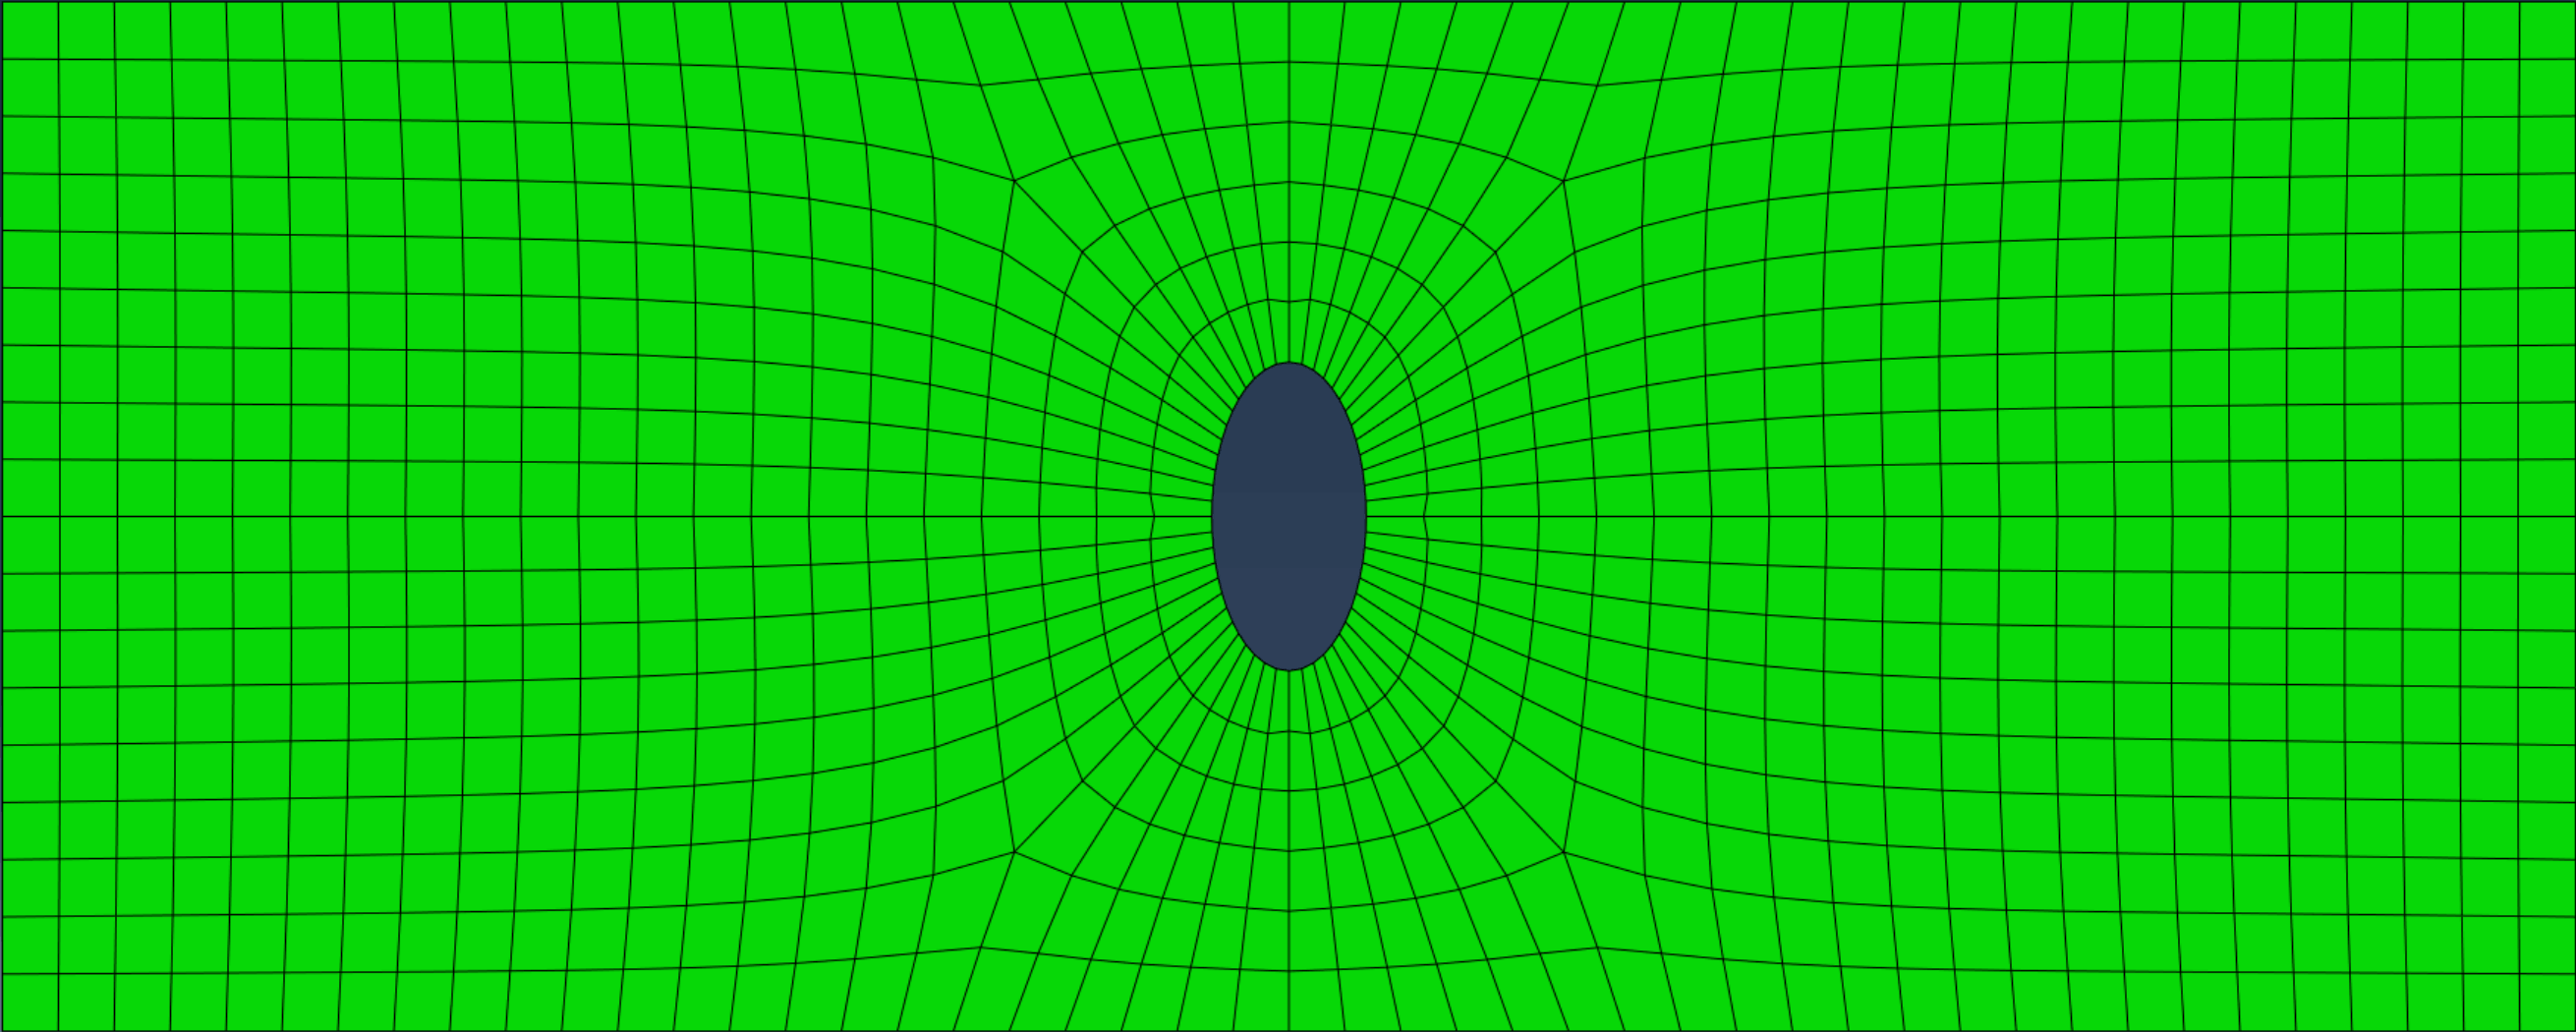
\includegraphics[width=\textwidth]{_ltx/Kuhn_A2-2_lin-seeded_mesh.png} % Datei für seeded mesh
        \caption{Mesh der Scheibe mit linearen Elementen und gesteuertem Seeding}
        \label{fig:lin-seeded_mesh}
    \end{subfigure}

    \vspace{.5em} % Optional: Zusätzlicher vertikaler Abstand zwischen den Bildern

    \begin{subfigure}{0.48\textwidth}
        \centering
        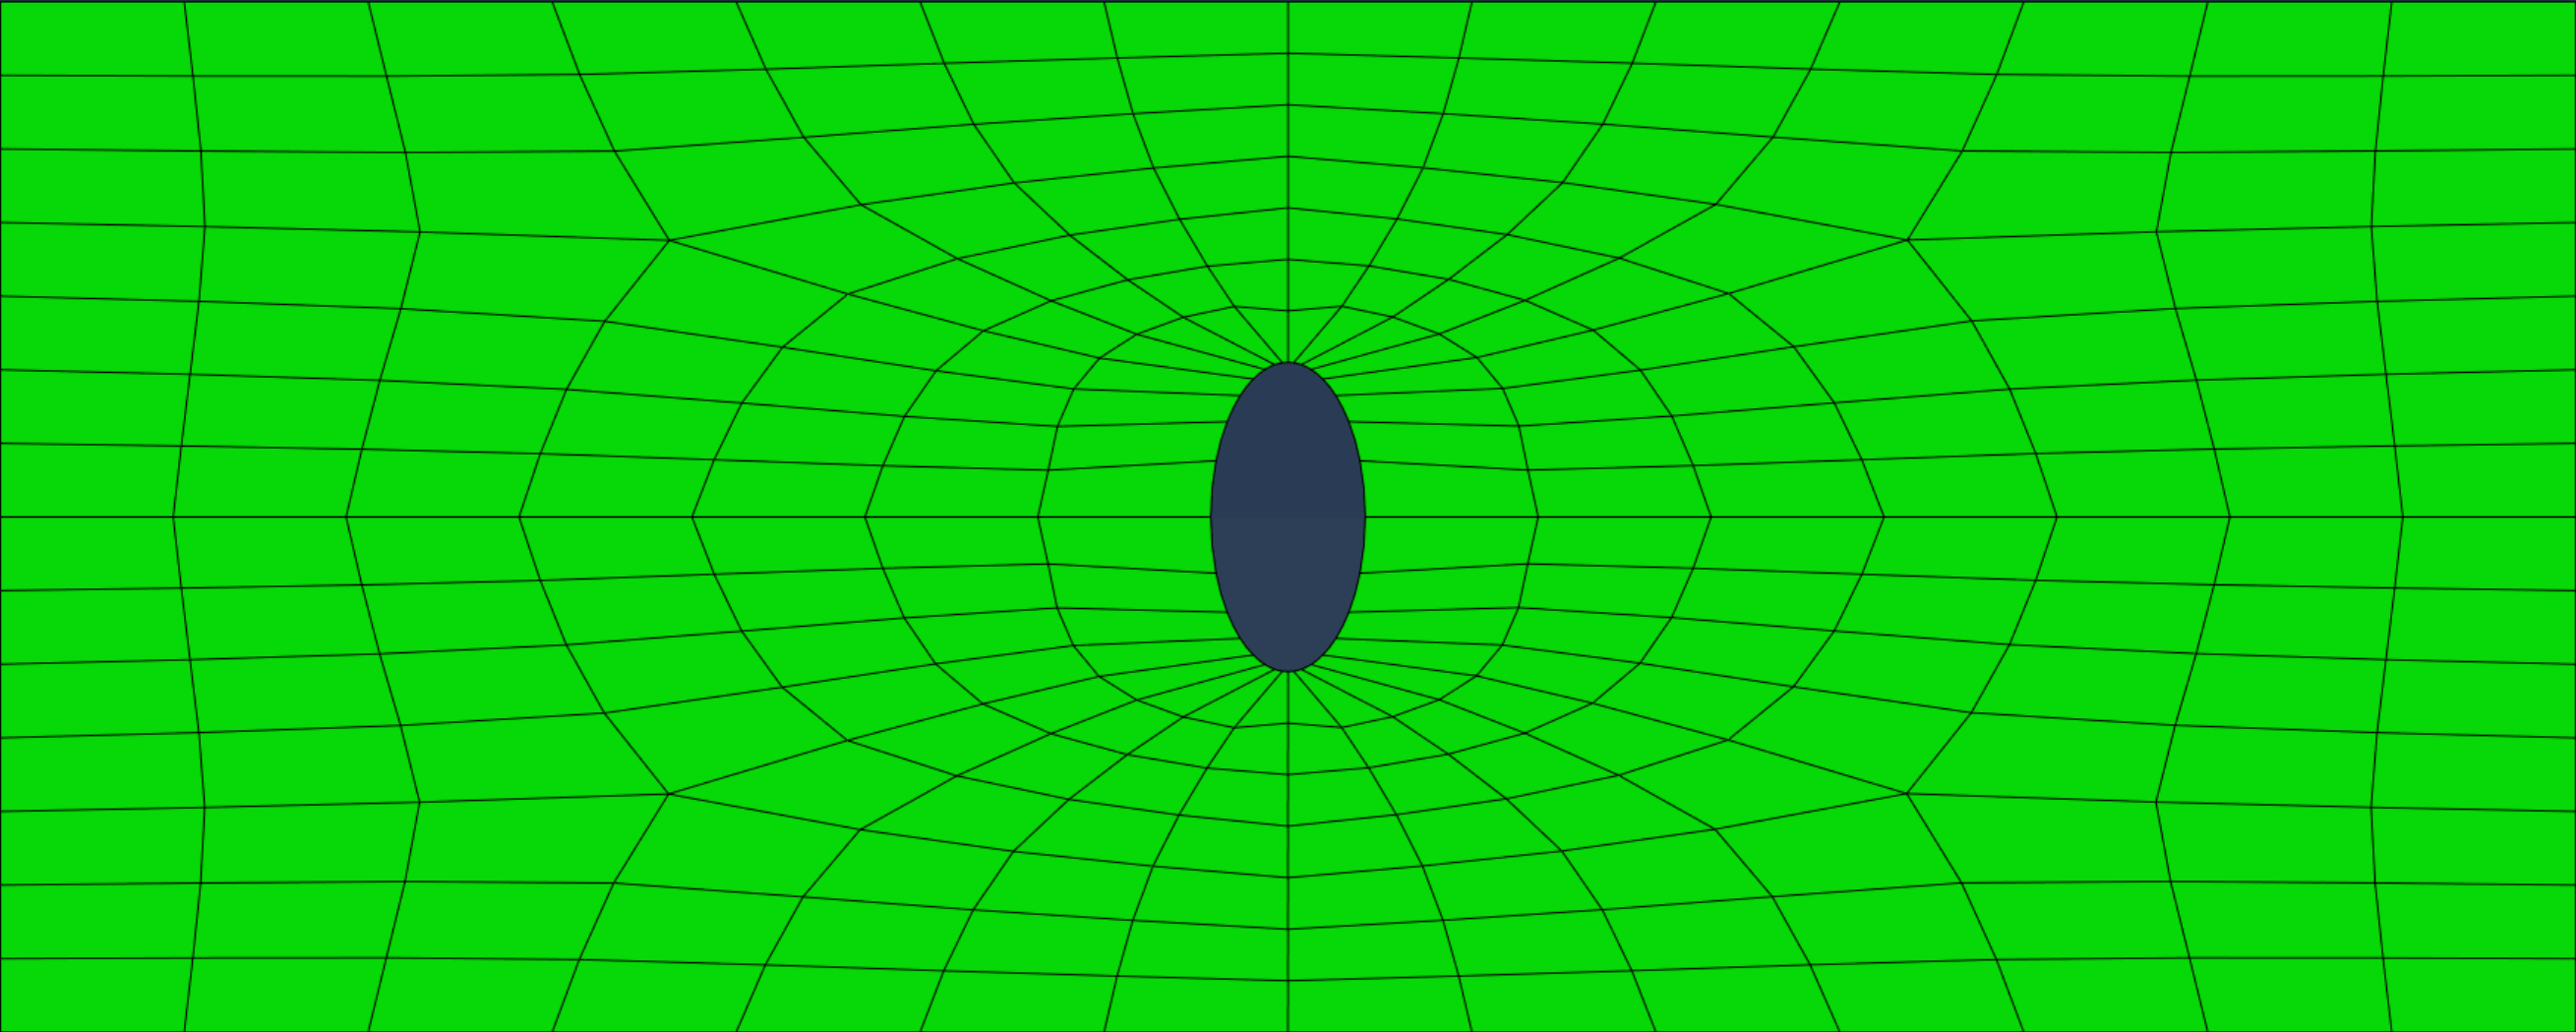
\includegraphics[width=\textwidth]{_ltx/Kuhn_A2-2_quad-seeded_V1_mesh.png} % Datei für quad seeded mesh V1
        \caption{Mesh der Scheibe mit quadratischen Elementen und gesteuertem Seeding V1}
        \label{fig:quad-seeded_V1_mesh}
    \end{subfigure}
    \hfill % Schiebt die Bilder auseinander, damit sie nebeneinander stehen
    %\vspace{.5em} % Optional: Zusätzlicher vertikaler Abstand zwischen den Bildern
    \begin{subfigure}{0.48\textwidth}
        \centering
        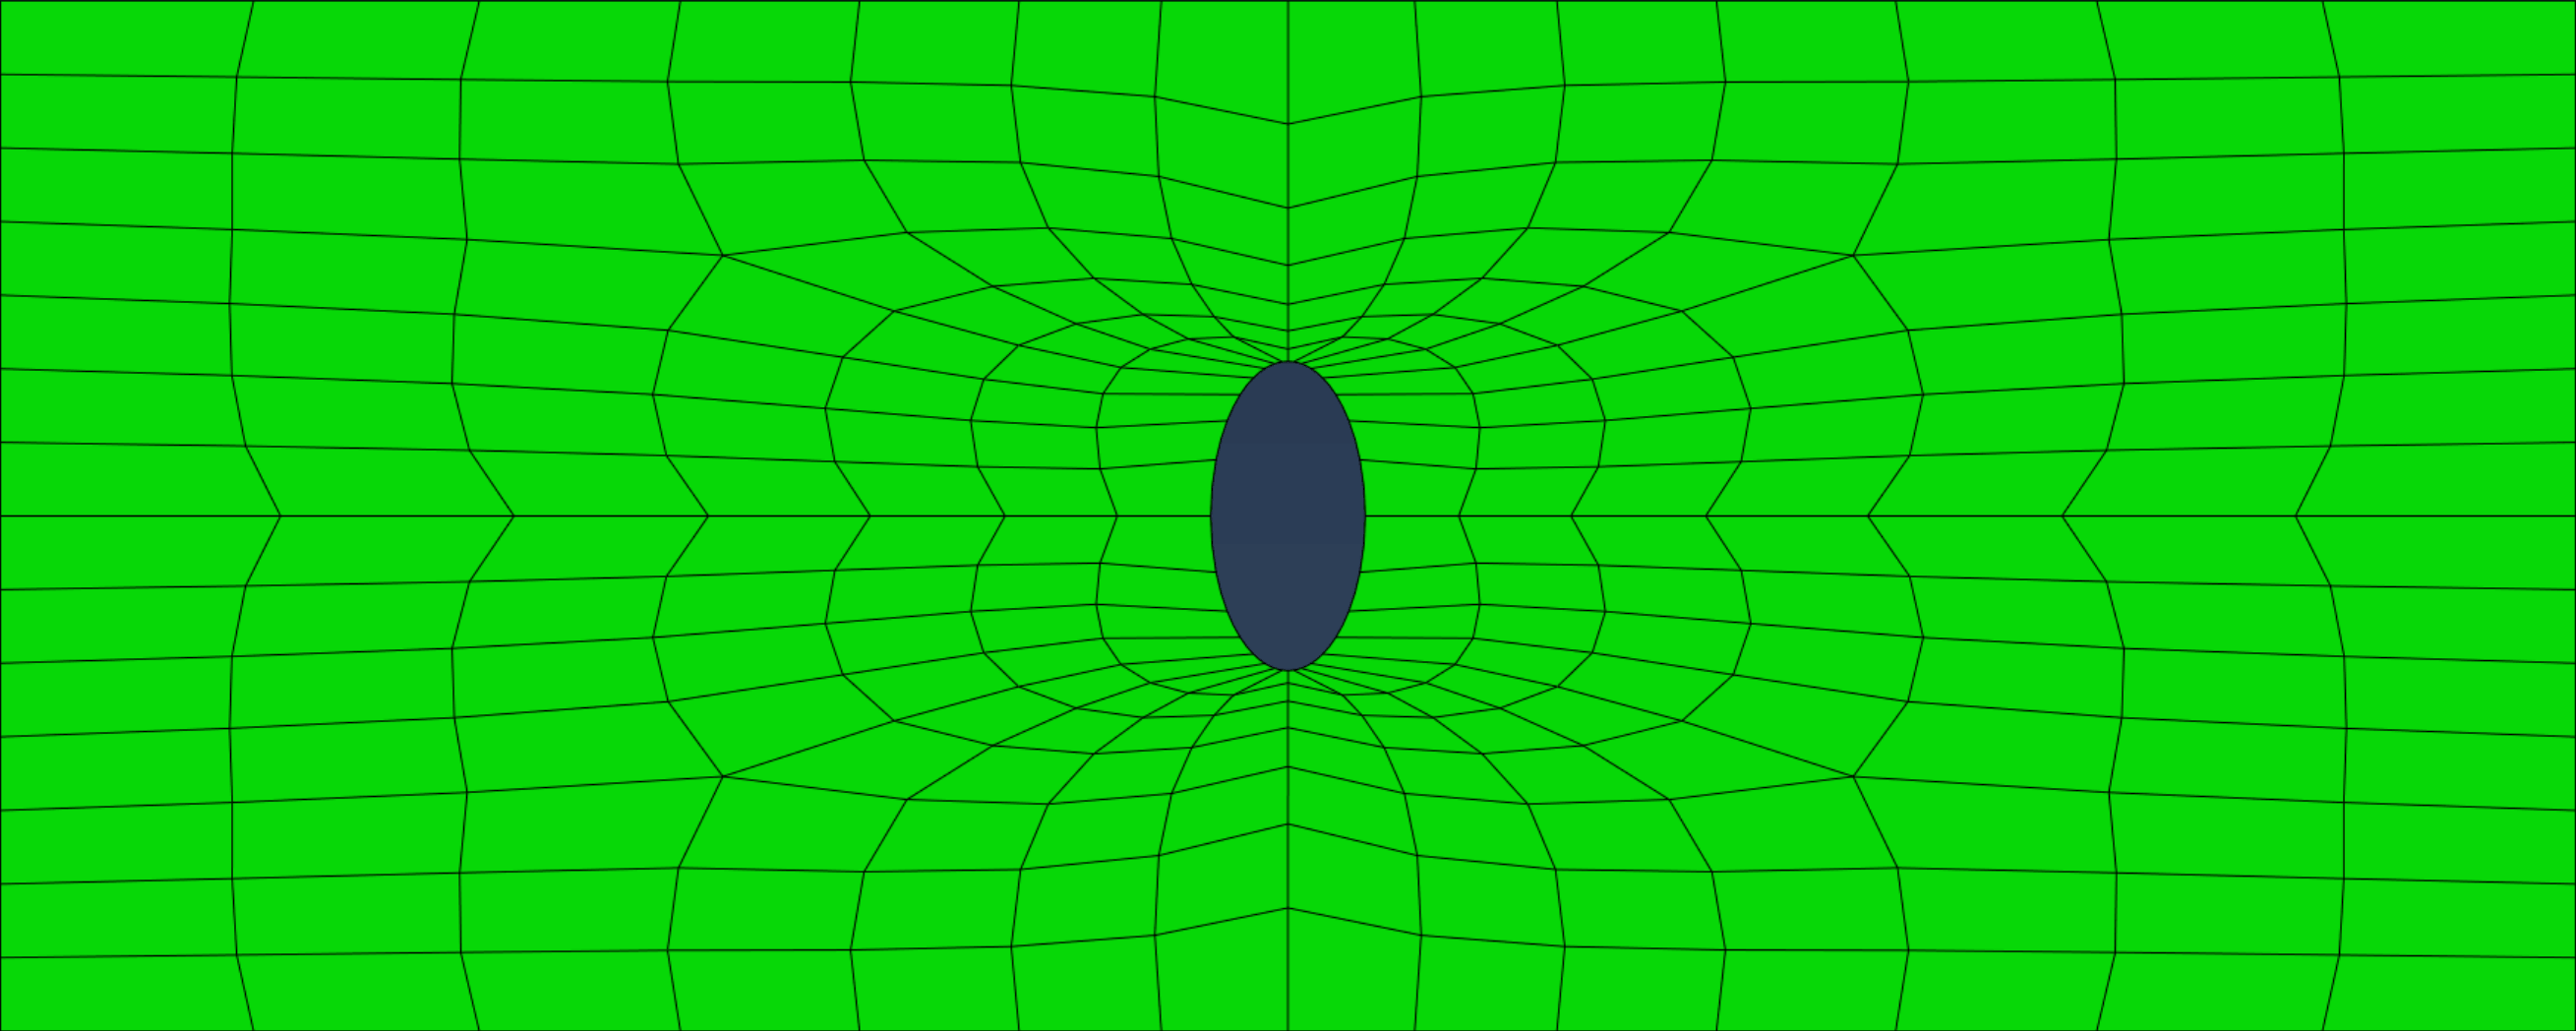
\includegraphics[width=\textwidth]{_ltx/Kuhn_A2-2_quad-seeded_V2_mesh.png} % Datei für quad seeded mesh V2
        \caption{Mesh der Scheibe mit quadratischen Elementen und gesteuertem Seeding V2}
        \label{fig:quad-seeded_V2_mesh}
    \end{subfigure}

    \caption{Mesh der Lochscheibe in den verschiedenen Iterationen der Netzoptimierung}
    \label{fig:Mesh Lochscheibe}
\end{figure}

\section{Pfaddefinition (Teilaufgabe \text{c)})}
\label{sec:Pfaddefinition}

Für die detaillierte Analyse des Spannungsverlaufs über die Scheibenhöhe wird ein vertikaler Auswertungspfad (Pfad $A-A$) definiert. Dieser Pfad liegt bei ${x = 50}$ über die gesamte Höhe der Scheibe. Entlang dieses Pfads werden die Normalspannungen ${\sigma_{xx}}$ extrahiert, um den Gradientenabbau ausgehend von der Kerbe in den ungestörten Bereich der Scheibe grafisch darzustellen und zu diskutieren.

%==== Kap4: ====
\chapter{Ergebnisse und Diskussion}
\label{sec:Ergebnisse und Diskussion}

In diesem Kapitel werden die Ergebnisse der analytischen Berechnungen nach Inglis mit der Finite-Elemente-Simulation verglichen, um die Genauigkeit des FE-Modells zu validieren. Im Folgenden werden die wichtigsten Erkenntnisse und Abweichungen diskutiert.

\section{Analytische Berechnungen}
\label{Analytische Berechnung}

Die theoretische Grundlage bildet die Lösung nach Inglis für eine unendlich ausgedehnte Scheibe. Unter Berücksichtigung der Halbachsen ${a = 6\,\mathrm{mm}}$ (vertikal) und ${b = 3\,\mathrm{mm}}$ (horizontal) sowie der Nennspannung ${\sigma_0 = 100\,\mathrm{MPa}}$ ergibt sich die maximale Kerbspannung am Lochrand zu:
\begin{equation}
    \sigma_{xx}^{\mathrm{P}} = 100\,\mathrm{MPa} \cdot \left( 1 + \frac{2 \cdot 6\,\mathrm{mm}}{3\,\mathrm{mm}} \right) = 500\,\mathrm{MPa}.
\end{equation}

\section{Vergleich der Diskretisierungsstrategien}
\label{sec:Vergleich der Diskretisierungsstrategien}

Die Simulationsergebnisse verdeutlichen die hohe Sensitivität der berechneten Spannungsspitzen gegenüber dem gewählten Mesh-Layout und der Elementformulierung.
\begin{itemize}
    \item \texttt{Kuhn\_A2-2\allowbreak \_lin-unseeded.odb}: Die Verwendung eines groben Netzes \sfigref{fig:lin-unseeded_S11} führt zu einer signifikanten Unterschätzung der Kerbspannung auf ca. ${425\,\mathrm{MPa}}$ (Abweichung von ${15\,\%}$). Die Detailansicht (\figref{fig:lin-unseeded_S11_detail}) zeigt eine stufige Darstellung der Spannungsgradienten, da die linearen Formfunktionen den steilen Abfall der Spannung im Kerbbereich nicht adäquat auflösen können.
    \item \texttt{Kuhn\_A2-2\_lin-seeded.odb}: Trotz der lokalen Verfeinerung am Lochrand (\figref{fig:lin-seeded_S11} und \figref{fig:lin-seeded_S11_detail}) verbessert sich das Ergebnis nur geringfügig auf ca. ${429\,\mathrm{MPa}}$. Dies belegt, dass bei hohen Spannungsgradienten und gekrümmten Geometrien eine reine Erhöhung der Elementanzahl bei linearen Elementen (ohne parabolische Formfunktionen) nur langsam zur Konvergenz führt.
    \item \texttt{Kuhn\_A2-2\_quad-seeded\_V1.odb}: Mit dem Wechsel auf voll integrierte quadratische Elemente \texttt{CPS8} und einem Bias-Seeding am Lochumfang wird ein Spitzenwert von ca. ${494\,\mathrm{MPa}}$ erreicht. (\sfigref{fig:quad-seeded_V1_S11}) Dies entspricht einer Abweichung von weniger als ${1.2\,\%}$ zum analytischen Wert. Die Detailansicht in \figref{fig:quad-seeded_V1_S11_detail} zeigt einen harmonischen, weichen Spannungsübergang, was auf eine hohe numerische Güte der Lösung hindeutet. Die geringe Restabweichung lässt sich auf den Einfluss der endlichen Plattenbreite im Vergleich zum unendlichen analytischen Modell zurückführen.
    \item \texttt{Kuhn\_A2-2\_quad-seeded\_V2.odb}: Durch eine Einführung des Single-Bias an den Quadrantenteilenden und Außenkanten (\sfigref{fig:quad-seeded_V2_S11}) steigt die Kerbspannung auf ca. ${627\,\mathrm{MPa}}$ (Abweichung von ca. ${25\,\%}$). Die Detailanalyse in \figref{fig:quad-seeded_V2_S11_detail} offenbart hier einen numerischen Fehler: Die Elemente an der Kerbspitze werden durch das extreme Seeding geometrisch so stark verzerrt, dass sie mathematisch kollabieren. Dies führt bei der Extrapolation von den Integrationspunkten zu den Knoten zu physikalisch unsinnigen Spannungsspitzen.
\end{itemize}

\begin{figure}
    \centering

    \begin{subfigure}{.55\textwidth}
        \centering
        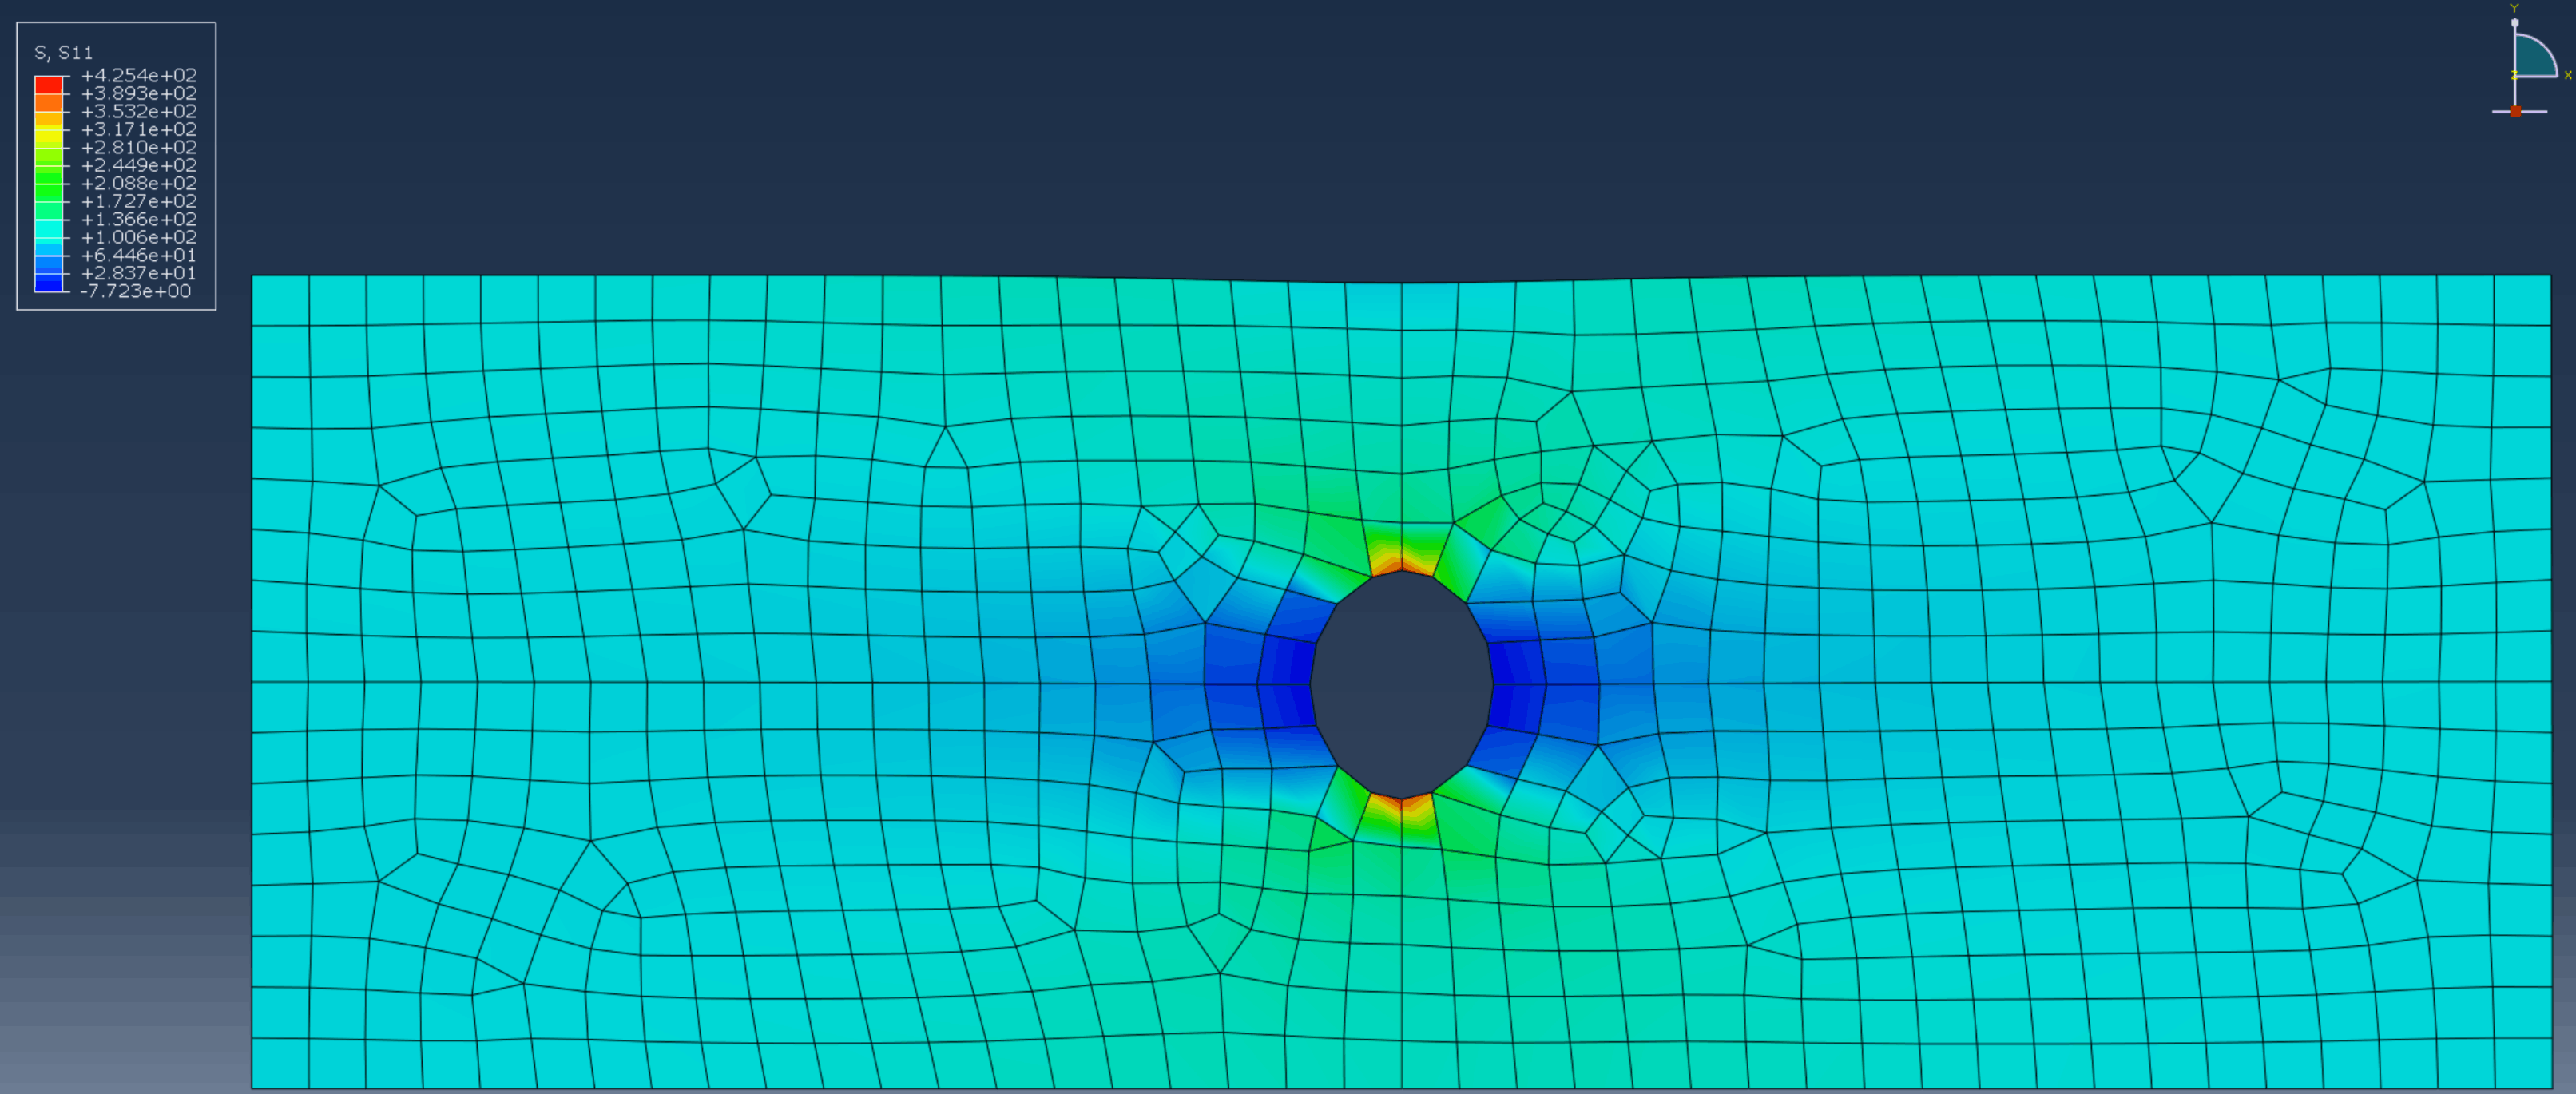
\includegraphics[width=\textwidth]{_ltx/Kuhn_A2-2_lin-unseeded_S11.png} % Datei für unseeded S11
        \caption{${S11}$ der Scheibe mit linearen Elementen und ungesteuertem Seeding}
        \label{fig:lin-unseeded_S11}
    \end{subfigure}

    %\hfill % Schiebt die Bilder auseinander, damit sie nebeneinander stehen
    \vspace{.5em} % Optional: Zusätzlicher vertikaler Abstand zwischen den Bildern
    \begin{subfigure}{.55\textwidth}
        \centering
        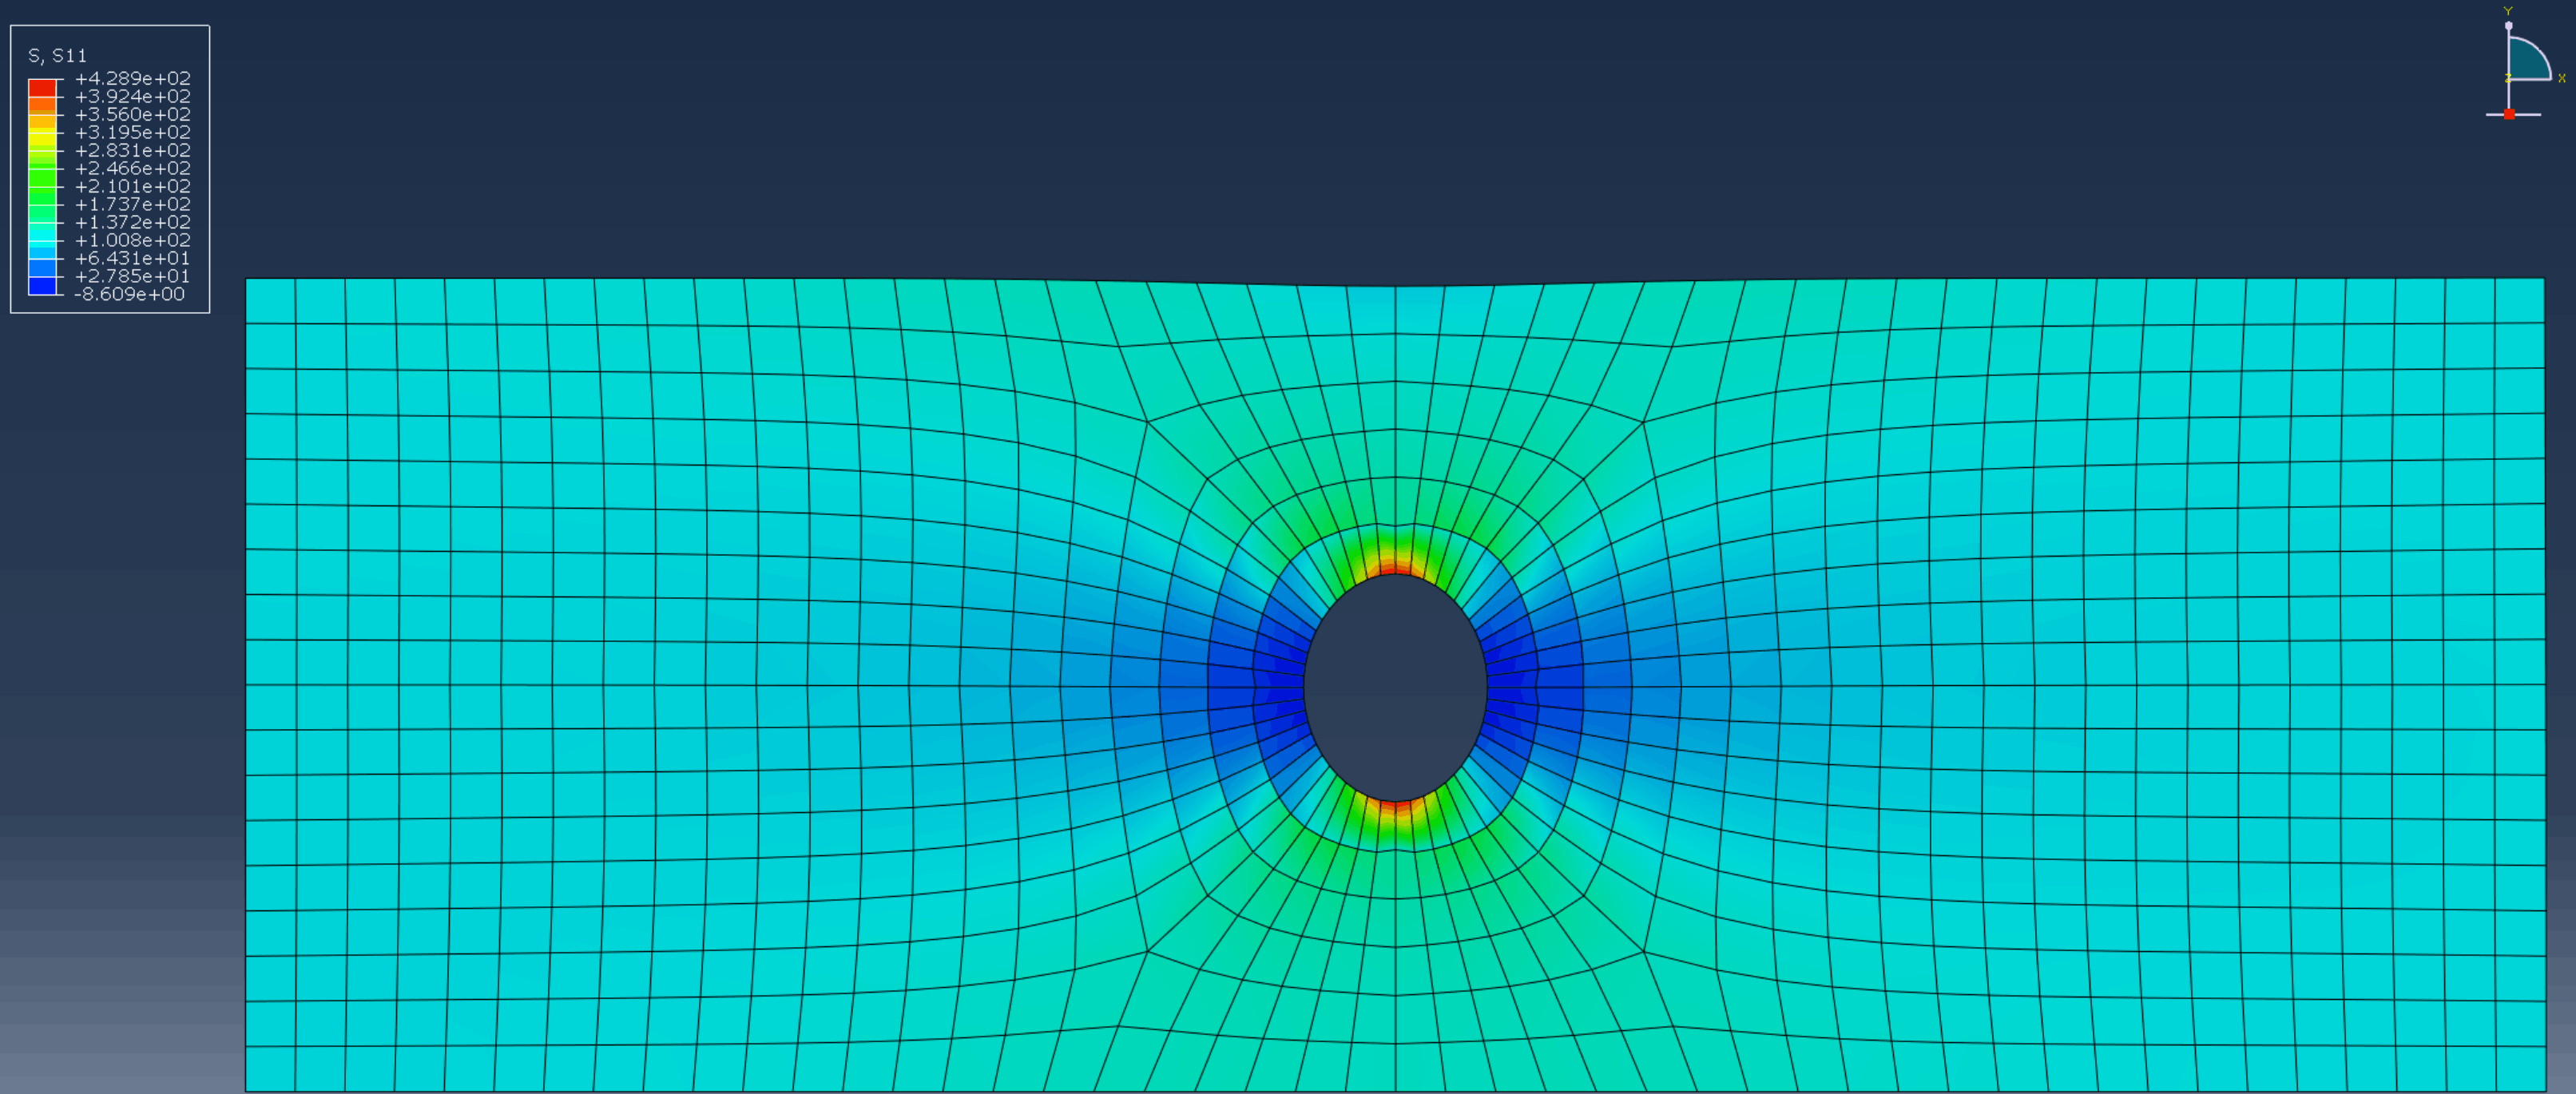
\includegraphics[width=\textwidth]{_ltx/Kuhn_A2-2_lin-seeded_S11.png} % Datei für seeded S11
        \caption{${S11}$ der Scheibe mit linearen Elementen und gesteuertem Seeding}
        \label{fig:lin-seeded_S11}
    \end{subfigure}

    \vspace{.5em} % Optional: Zusätzlicher vertikaler Abstand zwischen den Bildern

    \begin{subfigure}{.55\textwidth}
        \centering
        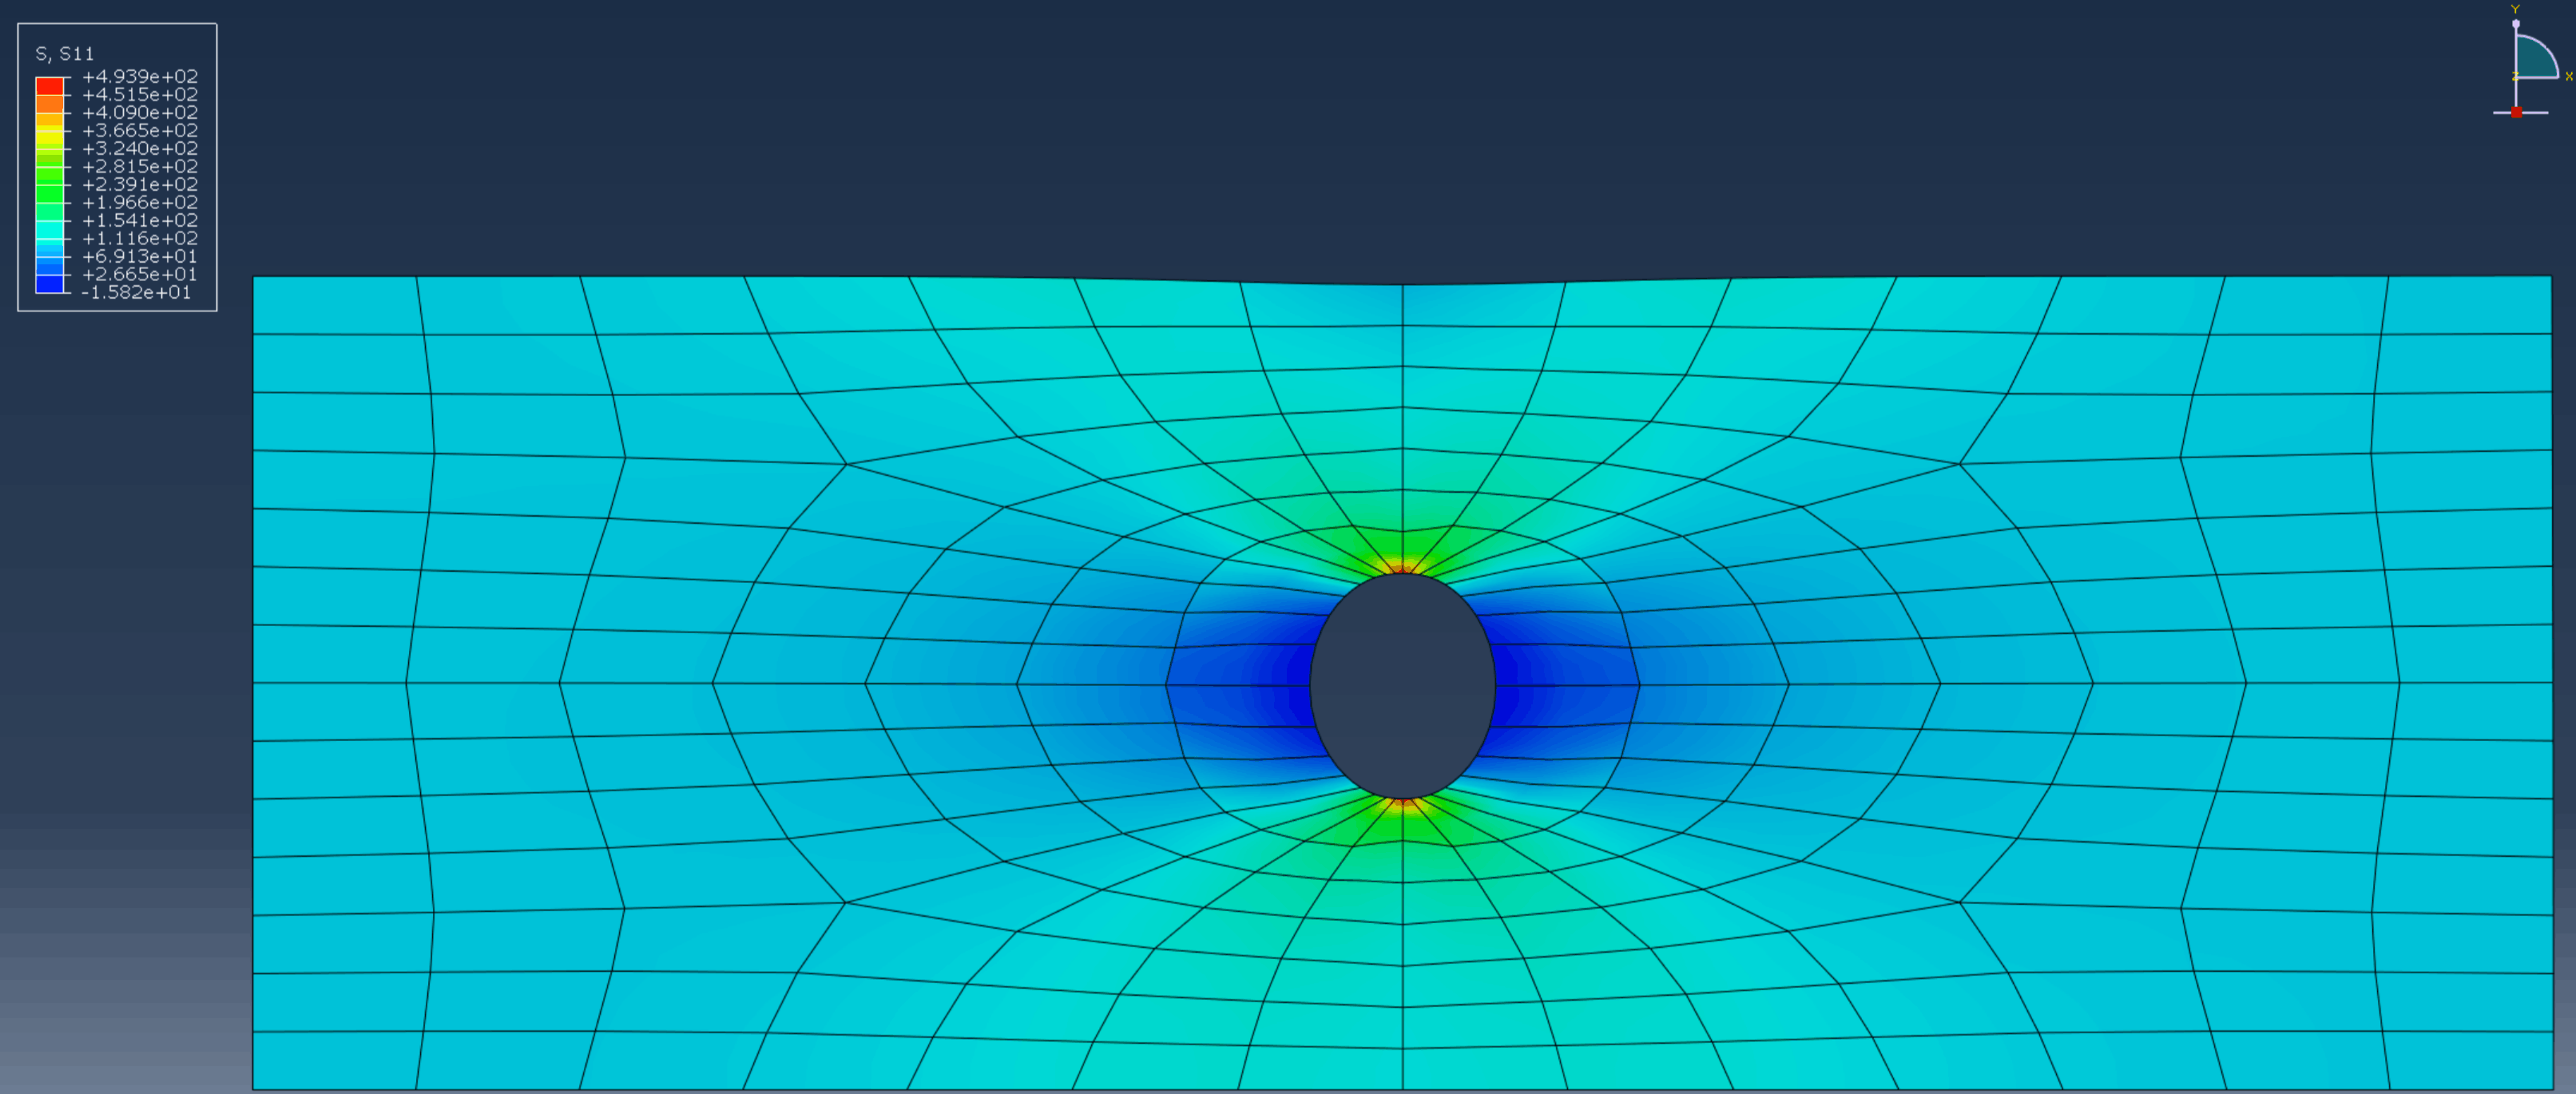
\includegraphics[width=\textwidth]{_ltx/Kuhn_A2-2_quad-seeded_V1_S11.png} % Datei für quad seeded mesh V1
        \caption{${S11}$ der Scheibe mit quadratischen Elementen und gesteuertem Seeding V1}
        \label{fig:quad-seeded_V1_S11}
    \end{subfigure}

    %\hfill % Schiebt die Bilder auseinander, damit sie nebeneinander stehen
    \vspace{.5em} % Optional: Zusätzlicher vertikaler Abstand zwischen den Bildern
    \begin{subfigure}{.55\textwidth}
        \centering
        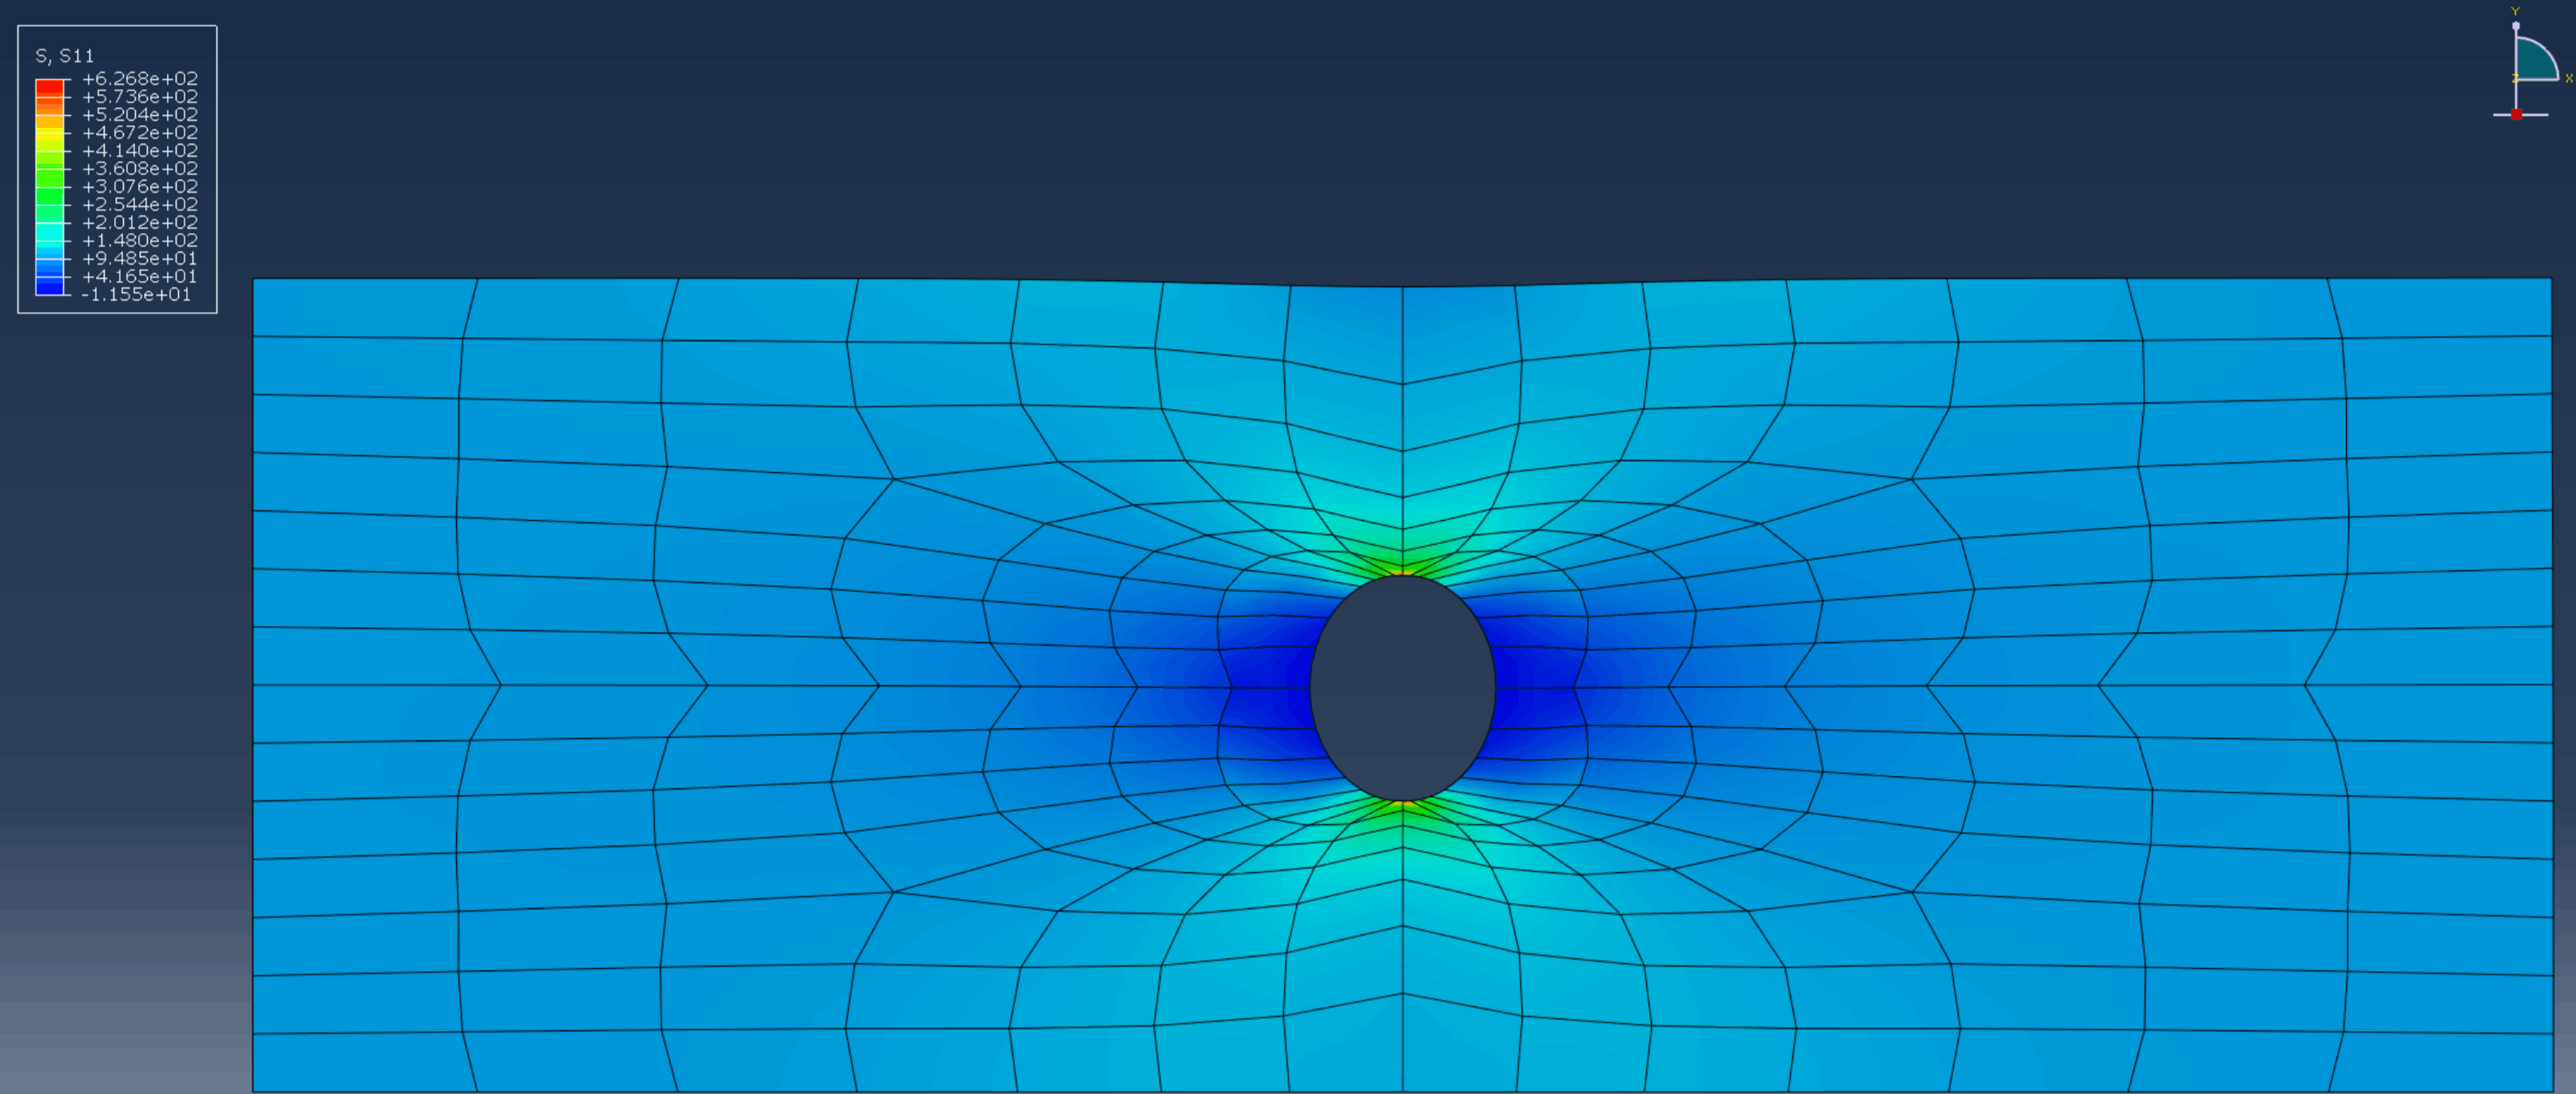
\includegraphics[width=\textwidth]{_ltx/Kuhn_A2-2_quad-seeded_V2_S11.png} % Datei für quad seeded mesh V2
        \caption{${S11}$ der Scheibe mit quadratischen Elementen und gesteuertem Seeding V2}
        \label{fig:quad-seeded_V2_S11}
    \end{subfigure}

    \caption{${S11}$ der Lochscheibe in den verschiedenen Iterationen der Netzoptimierung}
    \label{fig:S11 Lochscheibe}
\end{figure}

\begin{figure}[htbp]
    \centering

    \begin{subfigure}{0.48\textwidth}
        \centering
        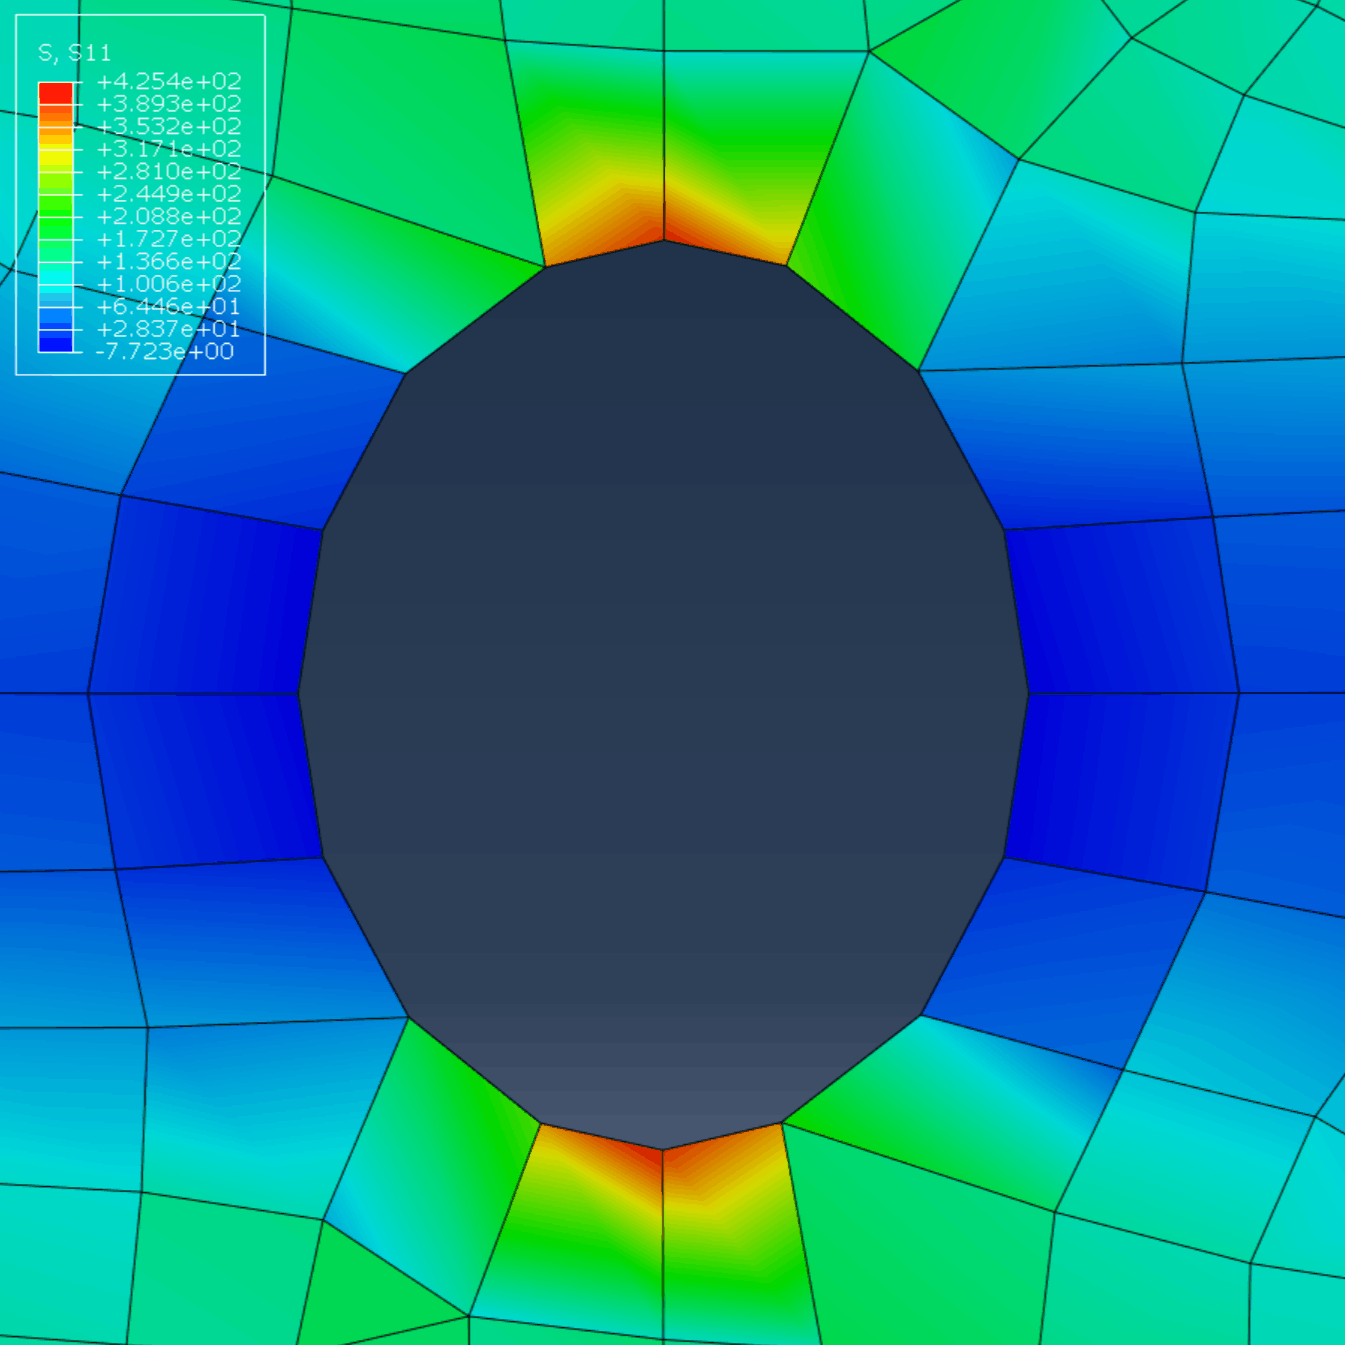
\includegraphics[width=\textwidth]{_ltx/Kuhn_A2-2_lin-unseeded_S11_detail.png} % Datei für unseeded S11 detail
        \caption{Detail ${S11}$ der Scheibe mit linearen Elementen und ungesteuertem Seeding}
        \label{fig:lin-unseeded_S11_detail}
    \end{subfigure}
    \hfill % Schiebt die Bilder auseinander, damit sie nebeneinander stehen
    %\vspace{.5em} % Optional: Zusätzlicher vertikaler Abstand zwischen den Bildern
    \begin{subfigure}{0.48\textwidth}
        \centering
        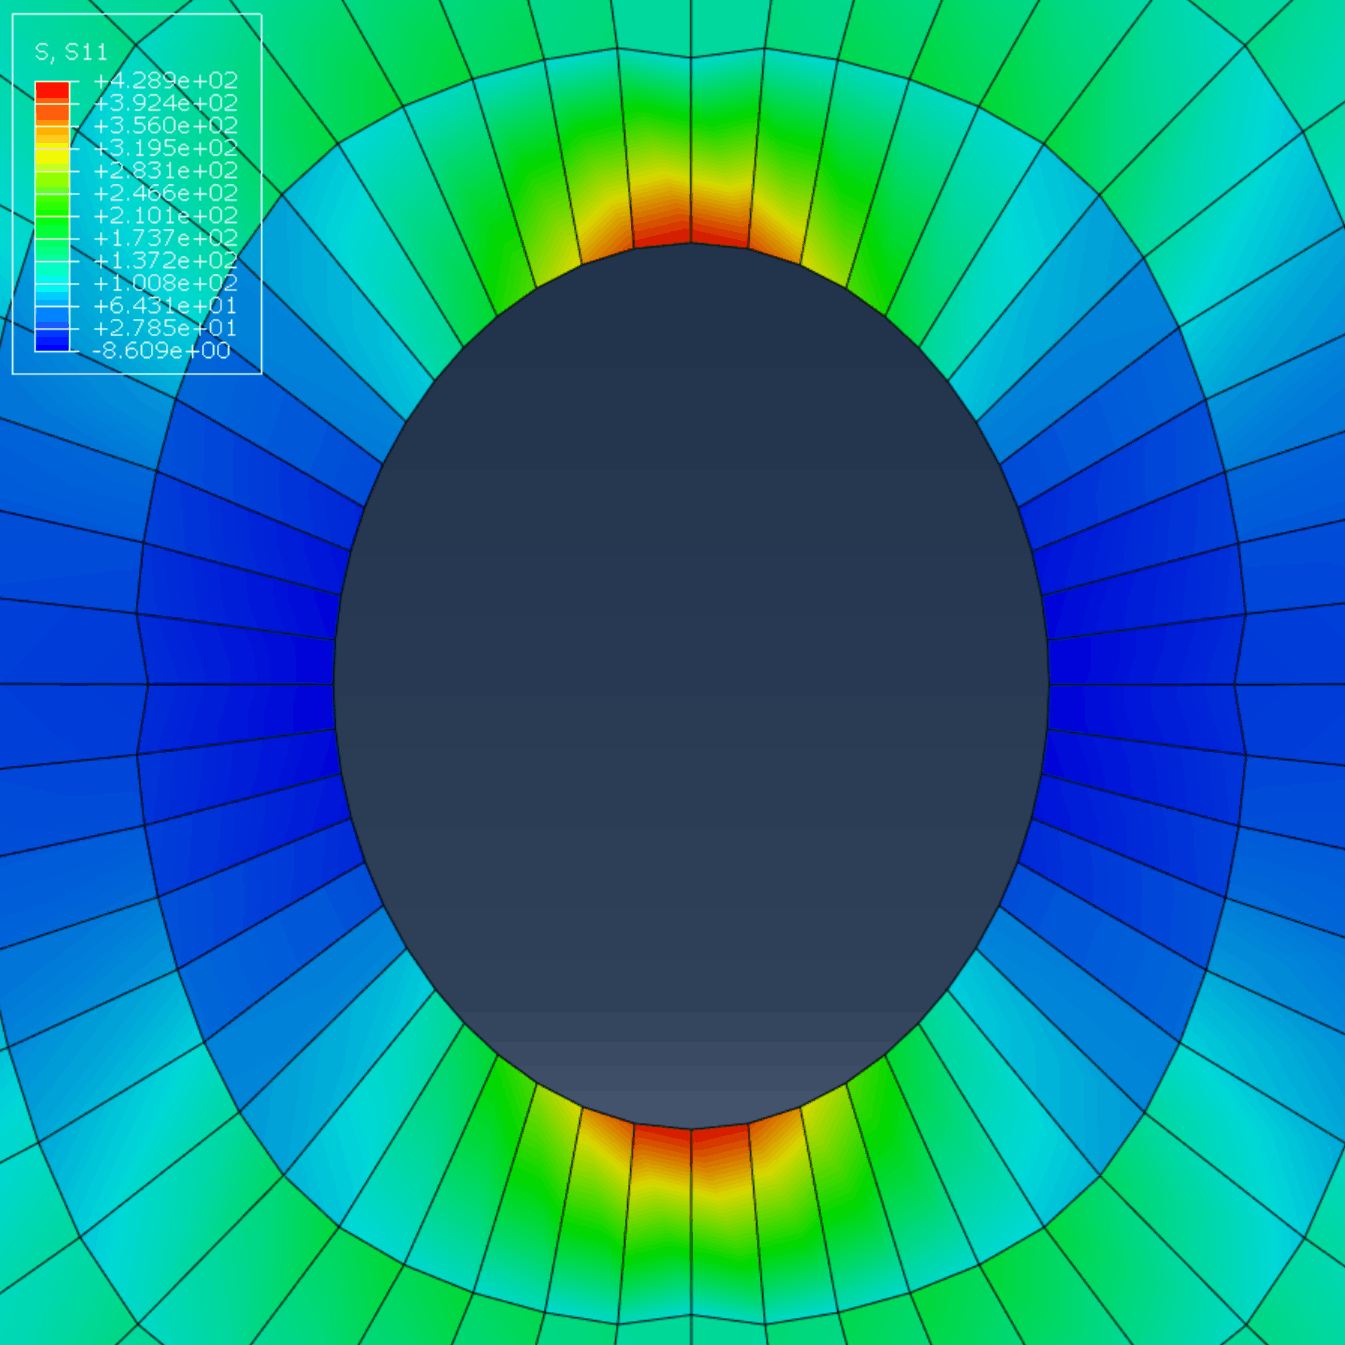
\includegraphics[width=\textwidth]{_ltx/Kuhn_A2-2_lin-seeded_S11_detail.png} % Datei für seeded S11 detail
        \caption{Detail ${S11}$ der Scheibe mit linearen Elementen und gesteuertem Seeding}
        \label{fig:lin-seeded_S11_detail}
    \end{subfigure}

    \vspace{.5em} % Optional: Zusätzlicher vertikaler Abstand zwischen den Bildern

    \begin{subfigure}{0.48\textwidth}
        \centering
        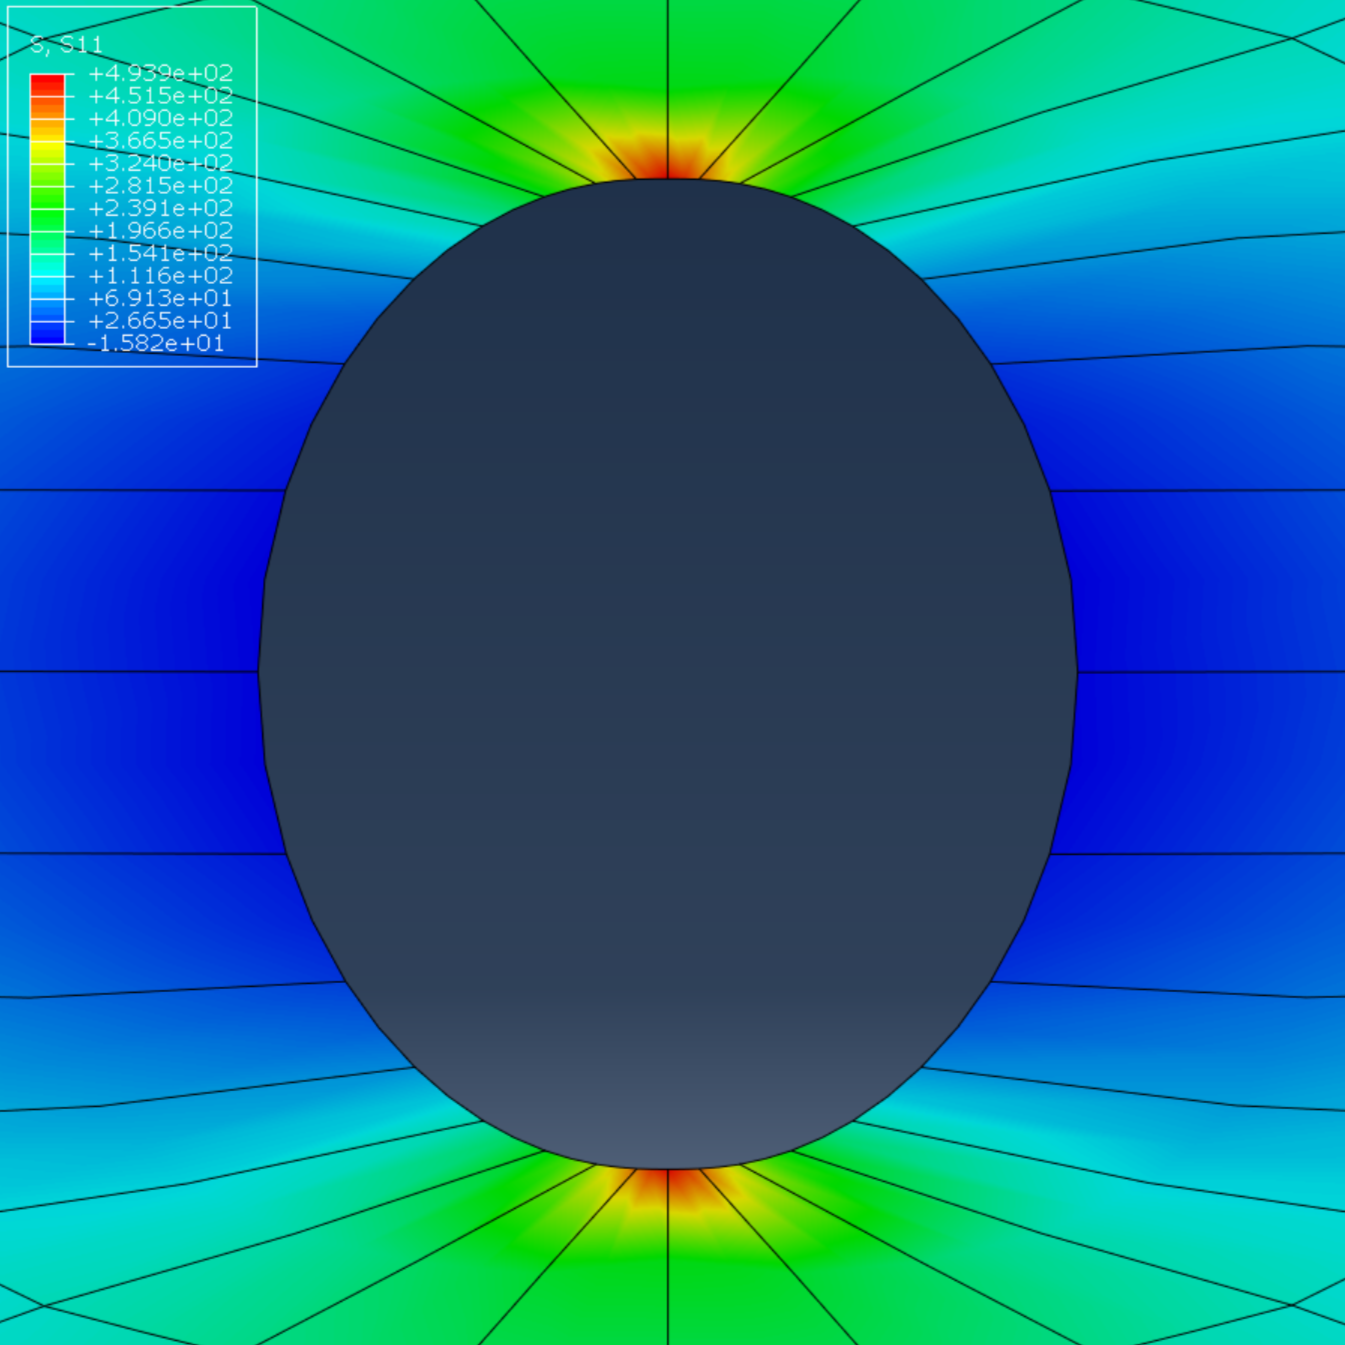
\includegraphics[width=\textwidth]{_ltx/Kuhn_A2-2_quad-seeded_V1_S11_detail.png} % Datei für quad seeded mesh V1 detail
        \caption{Detail ${S11}$ der Scheibe mit quadratischen Elementen und gesteuertem Seeding V1}
        \label{fig:quad-seeded_V1_S11_detail}
    \end{subfigure}
    \hfill % Schiebt die Bilder auseinander, damit sie nebeneinander stehen
    %\vspace{.5em} % Optional: Zusätzlicher vertikaler Abstand zwischen den Bildern
    \begin{subfigure}{0.48\textwidth}
        \centering
        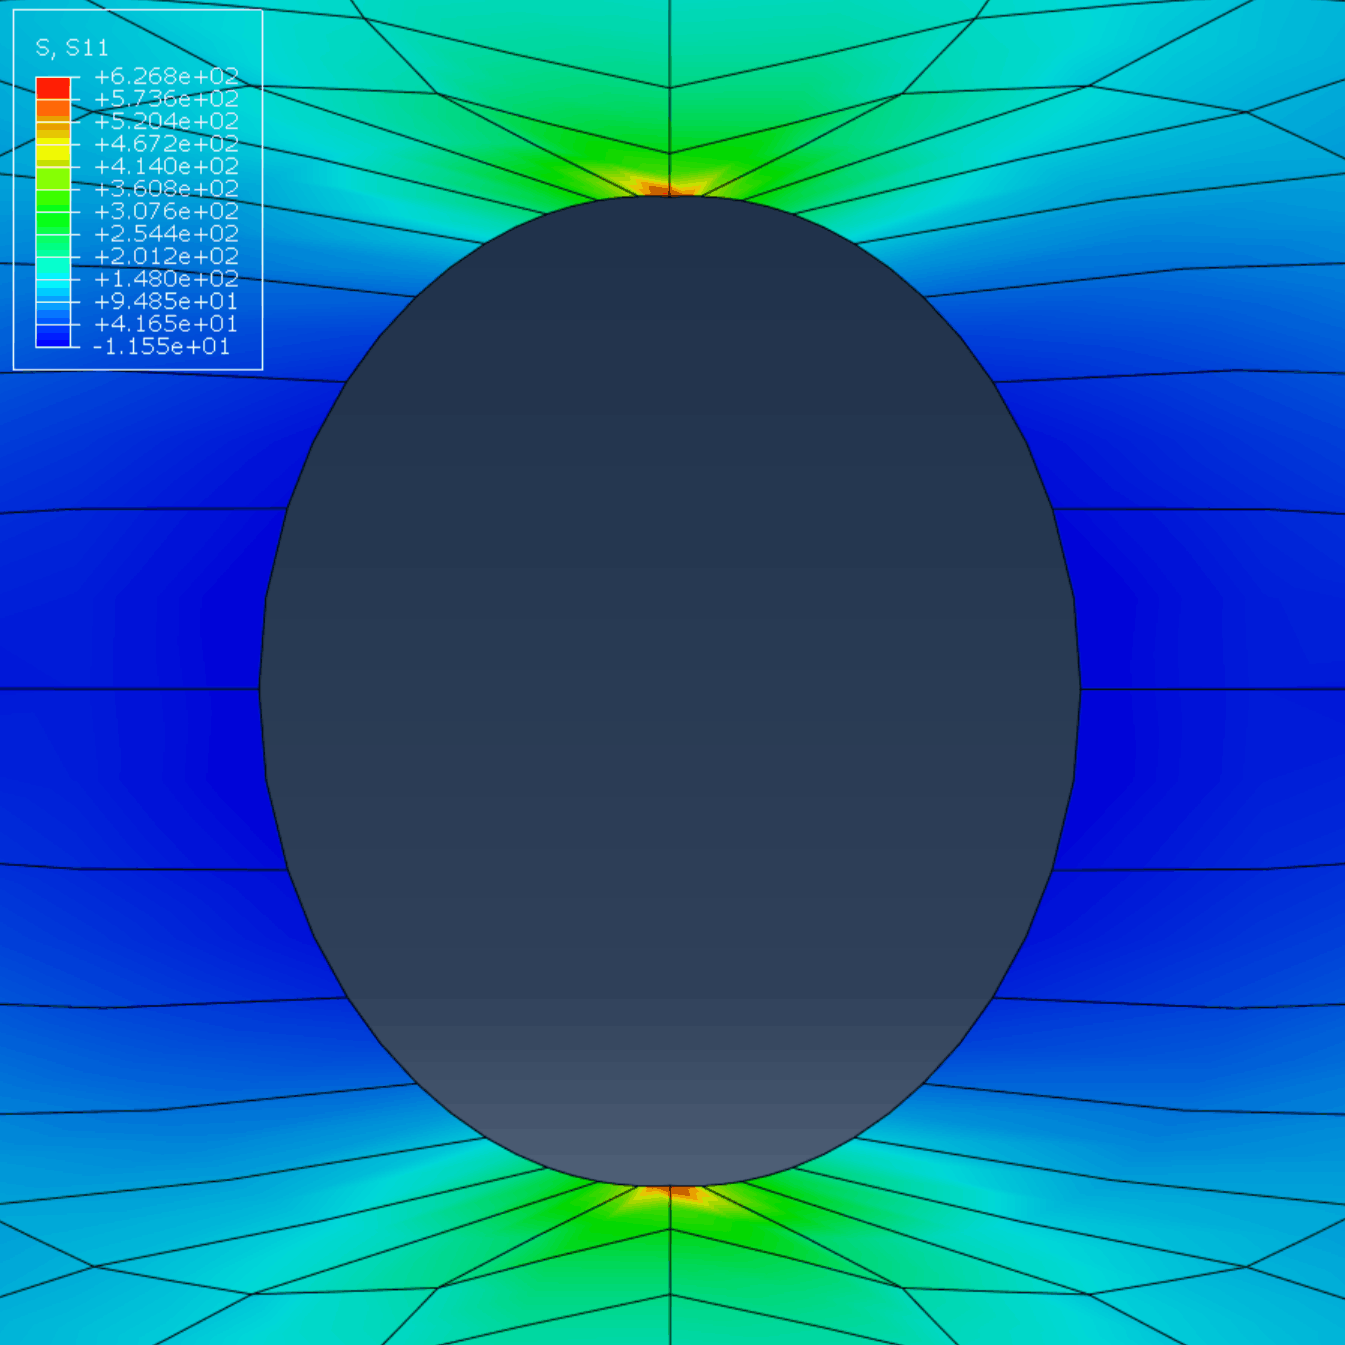
\includegraphics[width=\textwidth]{_ltx/Kuhn_A2-2_quad-seeded_V2_S11_detail.png} % Datei für quad seeded mesh V2 detail
        \caption{Detail ${S11}$ der Scheibe mit quadratischen Elementen und gesteuertem Seeding V2}
        \label{fig:quad-seeded_V2_S11_detail}
    \end{subfigure}

    \caption{Detailansicht ${S11}$ der Lochscheibe in den verschiedenen Iterationen der Netzoptimierung}
    \label{fig: Deatilansicht S11 Lochscheibe}
\end{figure}

\section{Analyse des Spannungsverlaufs entlang des Pfadplots ${A-A}$}
\label{sec:Analyse des Spannungsverlaufs entlang des Pfadplots A-A}

Der für die Version V1 generierte Pfadplot (\sfigref{fig:quad-seeded_V1_S11_path}) entlang des Pfads ${A-A}$ verdeutlicht den Charakter der Spannungskonzentration.
\begin{itemize}
    \item Kerbbereich: An den Scheitelpunkten des elliptischen Lochs (${y = 14\,\mathrm{mm}}$ und ${y = 26\,\mathrm{mm}}$) erreicht die Spannung ihr Maximum von ca. ${494\,\mathrm{MPa}}$.
    \item Gradientenabbau: Ausgehend vom Lochrand fällt die Spannung ${\sigma_{xx}}$ sehr steil ab. Bereits in geringer Entfernung zur Kerbe nähert sich der Verlauf dem ungestörten Spannungszustand an.
    \item Randbereich: An den Außenrändern der Scheibe (${y = 0\,\mathrm{mm}}$ und ${y = 40\,\mathrm{mm}}$) sinkt die Spannung auf Werte nahe der Nennspannung ${\sigma_0}$, was die lokale Begrenztheit des Kerbeinflusses (St. Venantsches Prinzip) bestätigt.
\end{itemize}

\begin{figure}[htbp]
    \centering
    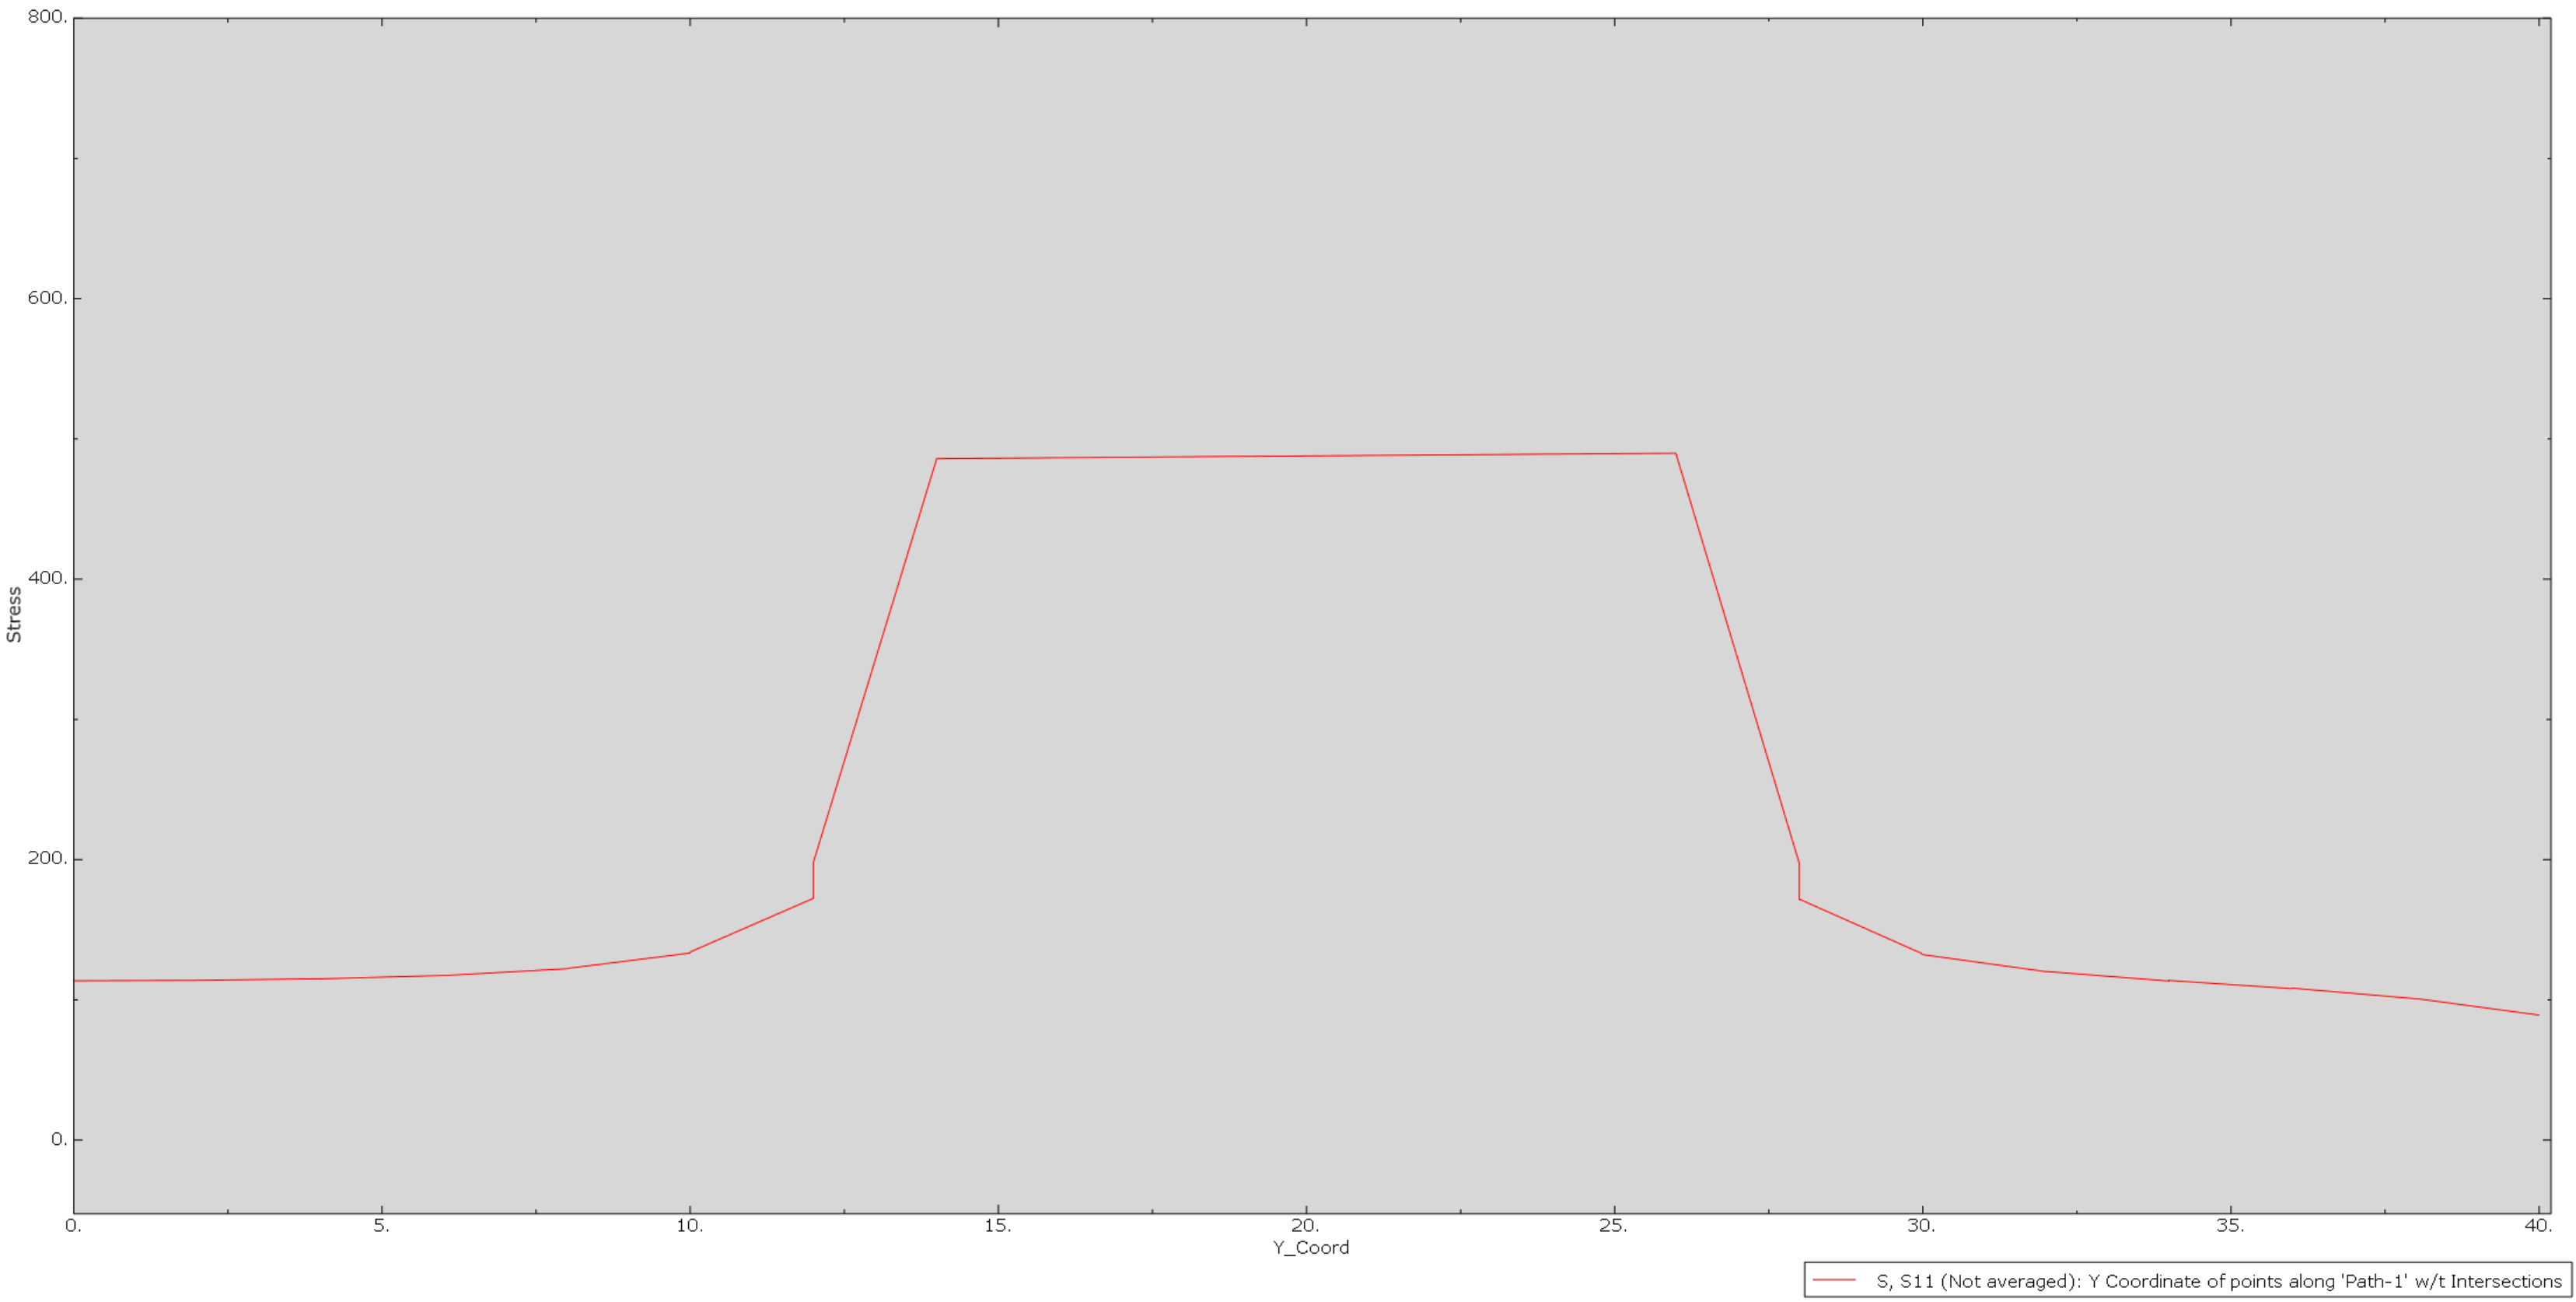
\includegraphics[width=\textwidth]{_ltx/Kuhn_A2-2_quad-seeded_V1_S11-path.png} % Datei für quad seeded S11 path
    \caption{Pfadplot ${A-A}$ der Scheibe mit quadratischen Elementen und gesteuertem Seeding V1}
    \label{fig:quad-seeded_V1_S11_path}
\end{figure}


%==== Kap4: ====
\chapter{Zusammenfassung und Fazit}
\label{sec:Zusammenfassung und Fazit}

\textbf{Zusammenfassung der Ergebnisse} \newline
Die vorliegende Arbeit demonstriert den Prozess der numerischen Spannungsanalyse an einer geometrischen Kerbe unter Einhaltung technischer Restriktionen. Durch die systematische Variation der Diskretisierungsparameter konnte die Überführung eines ungesteuerten Initialmodells in eine optimierte numerische Lösung vollzogen werden. Während das Ausgangsmodell mit linearer Elementformulierung und grobem Mesh die theoretische Kerbspannung von ${500\,\mathrm{MPa}}$ mit lediglich ca. ${425\,\mathrm{MPa}}$ signifikant unterschätzte, lieferte das optimierte Modell \texttt{Kuhn\_A2-2\_quad-seeded\_V1.odb} unter Verwendung quadratischer Elemente \texttt{CPS8} und radialem \texttt{Bias-Seeding} mit ${494\,\mathrm{MPa}}$ ein hochpräzises Ergebnis. Die verbleibende Differenz von ca. ${1.2\,\%}$ zum analytischen Wert nach Inglis lässt sich primär auf den physikalischen Einfluss der endlichen Plattenbreite zurückführen.

\textbf{Abschließendes Fazit und gewonnene Erkenntnisse} \newline
Aus der Problemlösung lassen sich drei zentrale Erkenntnisse für die ingenieurmäßige Simulationspraxis ableiten:
\begin{itemize}
    \item Überlegenheit quadratischer Elementformulierungen: In Bereichen mit hohen Spannungsgradienten, wie sie an Kerben auftreten, sind lineare Elemente aufgrund ihrer konstanten Dehnungsansätze oft zu steif (Locking-Effekte). Der Einsatz quadratischer Formfunktionen ist essenziell, um parabolische Spannungsverläufe und geometrische Krümmungen mit einer effizienten Anzahl an Knoten präzise abzubilden.
    \item Die Ambivalenz der Netzverfeinerung: Eine lokale Erhöhung der Knotendichte ist zur Auflösung von Gradienten zwingend erforderlich, darf jedoch nicht zu Lasten der Elementqualität gehen. Wie die Version V2 eindrucksvoll zeigt, führen extrem hohe Verfeinerungsgrade zu ungünstigen Seitenverhältnissen (Aspect Ratio), die mathematische Artefakte und physikalisch unmögliche Spannungsspitzen von über ${620\,\mathrm{MPa}}$ provozieren.
    \item Notwendigkeit der analytischen Plausibilisierung: Die Untersuchung unterstreicht, dass die numerische Simulation kein isoliertes Werkzeug ist. Ohne die Kenntnis der theoretischen Referenzlösung nach Inglis wäre Ergebnis \texttt{Kuhn\_A2-2\_quad-seeded\_V2.odb} möglicherweise als hochgenau missinterpretiert worden. Die Aufgabe des Ingenieurs besteht somit nicht nur in der Modellerstellung, sondern primär in der kritischen Validierung der Ergebnisse gegen theoretische Grenzwerte.
\end{itemize}
Durch die methodische Kombination aus gezielter Partitionierung, bewusster Elementwahl und kritischer Ergebniskontrolle konnte nachgewiesen werden, dass auch unter lizenzbedingter Limitierungen (1000-Knoten-Grenze) eine wissenschaftlich belastbare Lösung erzielt werden kann.

%==== Literaturverzeichnis ====
\clearpage
\phantomsection       % Wichtig, damit Verlinkungen im PDF richtig funktionieren
\addcontentsline{toc}{chapter}{\bibname} % Schreibt das Wort "Anhang" ins Inhaltsverzeichnis
\chapter*{\bibname}
\markboth{\bibname}{}
\insertbib
% In der Bib sollte für Normen und Richtlinien als Type MANUAL und Webseite als ONLINE eingegeben



%\phantomsection\label{sec:literaturverzeichnis}
%\bibliography{litbib}
%\addcontentsline{toc}{section}{\bibname}
%\clearpage

%=========================================================
%==== Anhang ====
\clearpage            % Sorgt dafür, dass der Anhang auf einer neuen Seite beginnt
\appendix             % Schaltet die Nummerierung von Zahlen (1,2) auf Buchstaben (A,B) um
\addtocontents{toc}{\protect\setcounter{tocdepth}{0}} % Ab hier nur noch die Chapter-Ebene (Ebene 0) ins Inhaltsverzeichnis aufnehmen, keine Sections (Ebene 1) mehr:
\chapter{Anhang}
\label{sec:Anhang}

\section{Abaqus .cae-file}
\label{sec:Abaqus .cae-file}

Das Abaqus .cae-file der Simulation ist im Anhang als separate Datei unter dem Dateiname: \verb+Kuhn_A2-2_03738470.cae+ beigefügt. Es enthält die vollständige Modellierung der Aufgabe 2.2.

\section{Abaqus .inp-files}
\label{sec:Abaqus .inp-files}

Die Abaqus .inp-files der Simulation sind im Anhang als separate Dateien unter den Dateinamen:
\begin{itemize}
    \item \verb+Kuhn_A2-2_lin-unseeded.inp+ (Teilaufgabe \text{a)} ohne seeding sowie linearen Elementen)
    \item \verb+Kuhn_A2-2_lin-seeded.inp+ (Teilaufgabe \text{b)} mit seeding um Loch ohne Bias sowie linearen Elementen)
    \item \verb+Kuhn_A2-2_quad-seeded_V1.inp+ (Teilaufgabe \text{b)} mit seeding um Loch mit single Bias sowie quadratischen Elementen)
    \item \verb+Kuhn_A2-2_quad-seeded_V2.inp+ (Teilaufgabe \text{b)} - mit seeding um Loch, radialen Führungslinien und Außenkanten sowie quadratischen Elementen)
\end{itemize}
beigefügt.

\section{Abaqus .odb-files}
\label{sec:Abaqus .odb-files}

Die Abaqus .odb-files der Simulation sind im Anhang als separate Dateien unter dem Dateiname:
\begin{itemize}
    \item \verb+Kuhn_A2-2_lin-unseeded.odb+ (Teilaufgabe \text{a)} ohne seeding sowie linearen Elementen)
    \item \verb+Kuhn_A2-2_lin-seeded.odb+ (Teilaufgabe \text{b)} mit seeding um Loch ohne Bias sowie linearen Elementen)
    \item \verb+Kuhn_A2-2_quad-seeded_V1.odb+ (Teilaufgabe \text{b)} mit seeding um Loch mit single Bias sowie quadratischen Elementen)
    \item \verb+Kuhn_A2-2_quad-seeded_V2.odb+ (Teilaufgabe \text{b)} - mit seeding um Loch, radialen Führungslinien und Außenkanten sowie quadratischen Elementen)
\end{itemize}
beigefügt.

\section{Abaqus .rpt-files}
\label{sec:Abaqus .rpt-files}

Die Abaqus .rpt-files der Simulation sind im Anhang als separate Dateien unter dem Dateiname:
\begin{itemize}
    \item \verb+Kuhn_A2-2_lin-unseeded.rpt+ (Teilaufgabe \text{a)} ohne seeding sowie linearen Elementen)
    \item \verb+Kuhn_A2-2_lin-seeded.rpt+ (Teilaufgabe \text{b)} mit seeding um Loch ohne Bias sowie linearen Elementen)
    \item \verb+Kuhn_A2-2_quad-seeded_V1.rpt+ (Teilaufgabe \text{b)} mit seeding um Loch mit single Bias sowie quadratischen Elementen)
    \item \verb+Kuhn_A2-2_quad-seeded_V2.rpt+ (Teilaufgabe \text{b)} - mit seeding um Loch, radialen Führungslinien und Außenkanten sowie quadratischen Elementen)
\end{itemize}
beigefügt.

\end{document}